\documentclass[a4paper]{article}
\usepackage{libertine}
\usepackage[T1]{fontenc}
\usepackage[utf8]{inputenc}
\usepackage{geometry}
\geometry{%
	left   = 3cm,
	right  = 3cm,
	top    = 3cm,
	bottom = 3cm
}
\usepackage{setspace}
\setstretch{1}
\usepackage{amsmath}
\usepackage{amssymb}
\usepackage[nolist]{acronym}
\usepackage{commath}
\usepackage{verbatim}
\usepackage{booktabs}
\usepackage{listings}
\usepackage{enumitem}
\usepackage{graphicx,color,psfrag}
% \usepackage{subfigure}
\usepackage{subcaption}
\usepackage{wrapfig}
\usepackage{svg}
\usepackage{svg-extract}
\usepackage{todonotes}
\usepackage[acronym,nonumberlist,nowarn,style=long]{glossaries}
\usepackage{color}
\usepackage{tikz}
\usepackage{pgf-umlsd}
\usepackage{ifthen}
\usepackage{hyperref}
\usepackage[binary-units]{siunitx}
\usepackage{bytefield}


%% List of Acronyms

\newacronym{acr:FPGA}{FPGA}{field programmable gate array}
\newacronym{acr:IP}{IP}{intellectual property}
\newacronym{acr:ILA}{ILA}{integrated logic analyzer}
\newacronym{acr:CNN}{CNN}{convolutional Neural Network}
\newacronym{acr:DMA}{DMA}{direct memory access}
\newacronym{acr:PS}{PS}{processing system}
\newacronym{acr:PL}{PL}{programmable logic}
\newacronym{acr:BRAM}{BRAM}{block-RAM}
\newacronym{acr:LUT}{LUT}{Look Up Table}
\newacronym{acr:NN}{NN}{neural network}
\newacronym{acr:DL}{DL}{deep learning}
\newacronym{acr:ML}{ML}{machine learning}
\newacronym{acr:GUI}{GUI}{graphical user interface}
\newacronym{acr:API}{API}{application programmable interface}


\newcommand{\stdlogic}{std\_logic}

\begin{document}
% This is used to limit the number of authors
% Unfortunatly only working on IEEE
% \bstctlcite{IEEEexample:BSTcontrol}

\begin{titlepage}
	
	\begin{flushright}
		
		% Update this with your team number]
		
		% Update this with your matriculation number, first name, second name
		\Large 
		Yellow Of The Egg\\
		\large
		Lukas Baischer	\\
		Benjamin Kulnik	\\
		Anton Leitner \\
		Stefan Marschner \\
		Miha Cerv \\
		
	\end{flushright}
	
	\vspace{5em}
	
	\begin{center}
		{\Large SoC Design Laboratoy}\\[1em]
		{\large 384.157, Winter Term 2019} \\[5em]

		
		{\Huge MNIST-FPGA\\[.5em]
		\huge Documentation}\\[10em]
	\end{center}

\end{titlepage}


\begin{acronym}
	\acro{FPGA}{Field Programmable Gate Array}
	\acro{FIFO}{First In, First Out}
	\acro{CNN}{Convolutional Neural Network}
\end{acronym}


\tableofcontents
\clearpage

\section{Introduction}

\subsection*{Notation}
\begin{center}
\begin{tabular}{lp{3.5in}}
	Weights 	& the parameter of the neural network		\\
	Activations	& the input and output values of the layers	\\
	Activation Function & Function that is applied at the output of a layer \\
	ReLU		& Rectified Linear Unit, defined as  $f(x) = \begin{cases}
		x \quad \text{if} \quad x > 0 \\
		0 \quad \text{else}
	\end{cases}$						\\
	Mini-Batch	& A small fraction of the input data \\
	Dense (Layer) & A layer where each neuron is connected to every input neuron \\
	Fully-Connected (Layer) & Same as \emph{Dense} 		\\
	$Q$			& The significant of a fix point integer 	\\
	$m$			& the exponent of a fix point integer		
\end{tabular}
\end{center}

\section{Concept}

\subsection{Neural Network}

For the neural network we base the architecture of our network on the well known \emph{LeNet} architecture from \cite{LeCun:1998aa} is chosen due to its simplicity and ease to implement. Additionally the performance is improved by using modern, established techniques like batch normalization \cite{Ioffe:2015aa} and dropout \cite{Srivastava:2014aa} layers. 
The training of network is done using PyTorch \cite{Paszke:2019aa} on a regular PC and the trained network parameters are then used to create a hardware VHDL model of the network. An overview of the structure can be seen in Figure~\ref{fig:eggnet}. For verification all neural network operations are checked in separate programmed programs for correctness. See the Section~\ref{subsec:nntraining} for details how the network is implemented in Software.
An excellent overview in deep learning can be found in \cite{Schmidhuber:2015aa} and also in \cite{Goodfellow:2016aa}.
To train and test the network we chose the MNIST dataset \cite{LeCun:1998ab}. It consists of 50.000 training images and 10.000 test images of handwritten digits, where each is 28-by-28 pixel.

\begin{figure}[hbt]
	\centering
	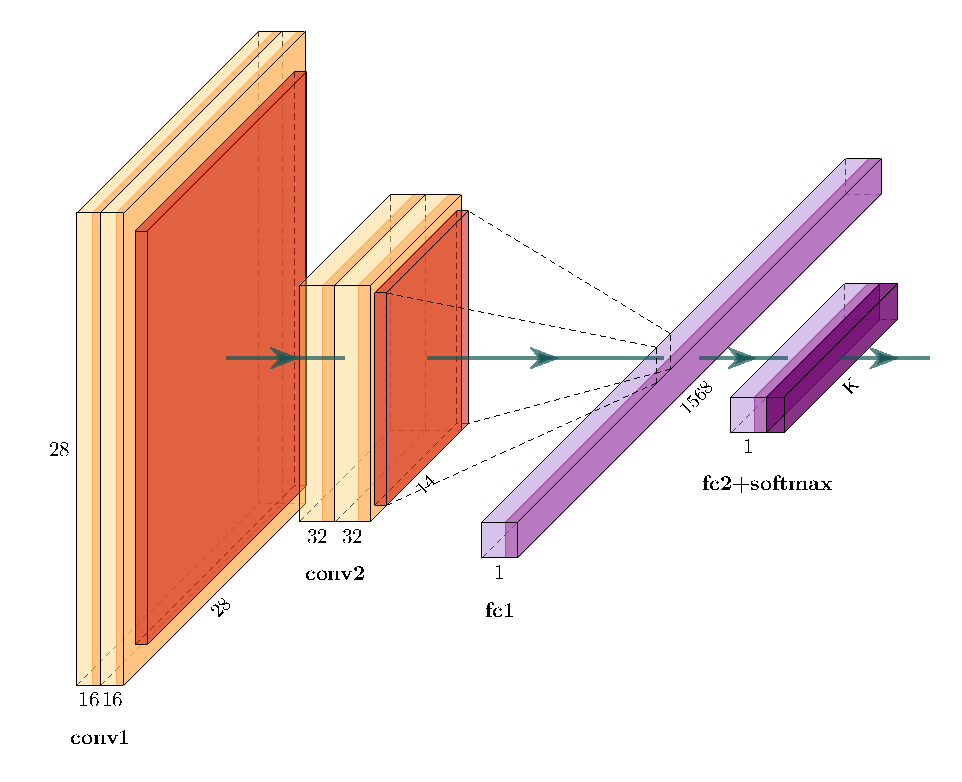
\includegraphics[width=0.6\textwidth]{img/eggnet}
	\caption{The Eggnet structure}
	\label{fig:eggnet}
\end{figure}


\subsection{Hardware Concept}
\begin{figure}[h]
	\centering
	\includesvg[width=0.8\textwidth]{img/inkscape/NN-concept.svg}
	\caption[Top-Level concept.]{Top-Level concept}
	\label{fig:hw-concept}
\end{figure}
\noindent
Figure \ref{fig:hw-concept} shows the Concept of implementing an FPGA-based hardware accelerator for handwritten digit recognition. A Zedboard is used as hardware platform, which includes a Zynq-7000 FPGA and provides various interfaces. It is also shown that the design can be remote controlled via a server which is running on the Zedboard. \\
A hardware accelerator for the neural network is implemented in the programmable logic part of the Zynq-7000. It is pre-trained using the remote PC, therefore only the inference of the neural network is implemented in hardware. \\
In order to train the network with the same bit resolution as implemented in the hardware, a software counterpart of the hardware is implemented in a PC using python. 
Based on the weights calculated by the python script a bitstream for the hardware is generated. This brings the benefit that for the convolutional layer constant multiplier can be used, since the weights of convolutional layer kernels are constant. For the dense layer it is not possible to implement the weights in a constant multiplier because in a dense layer each connection of a neuron requires a different weight, which would result in a huge amount of required constant multipliers. Therefore the weights for the dense layer have to be stored in a ROM inside the FPGA.   \\




\section{Neural Network Design and Training}
\label{subsec:nntraining}

%\begin{wrapfigure}{r}{0.5\textwidth}
%	\centering
%    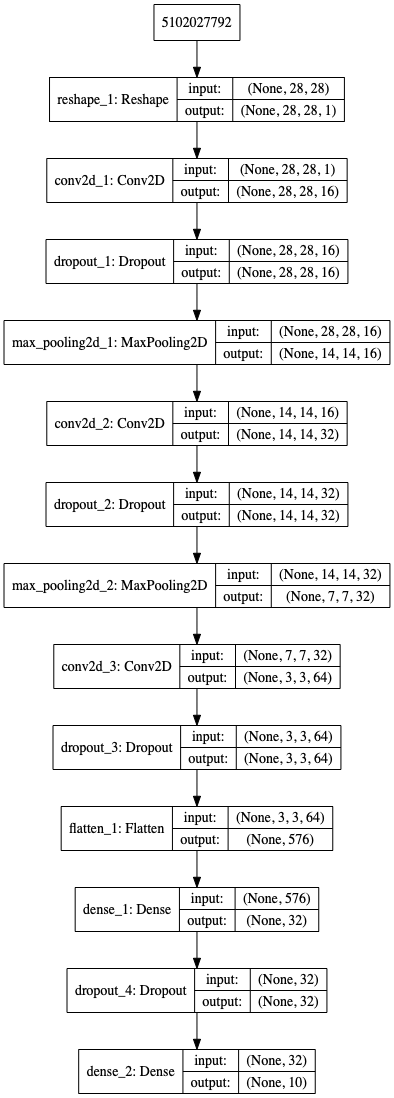
\includegraphics[width=0.35\textwidth]{img/nnlayout}
%	\caption{Network Layers}
%	\label{fig:network-layers}
%\end{wrapfigure}

The network was implemented in PyTorch \cite{Paszke:2019aa} as well as Tensorflow \cite{MartinAbadi:2015aa}. The backend was later exclusively switched to PyTorch (which is also the most common deep learning framework in Science) due to its better support of qunatization. The layers of the network can be seen in Figure~\ref{fig:network-layers}. 
For training of the network the \emph{ADAM} optimization algorithm \cite{Kingma:2014aa} was used to minimize the cross-entropy-loss function which is defined as
\begin{equation}
    J = - y  \log(h) + (1-y)  \log(1-h)
\end{equation}
For controlling the ADAM algorithm the recommended values, listed in Table~\ref{tab:train-params}, by \cite{Kingma:2014aa} was used.
\begin{table}[ht]
	\centering
    \caption{Network Training Parameters}
    \begin{tabular}{cc}
        \toprule
            Parameter & Value \\
        \midrule
            $\alpha$   & $0.001$ \\
            $\beta_1$  & $0.9$   \\
            $\beta_2$  & $0.999$  \\          
        \bottomrule
    \end{tabular}
    \label{tab:train-params}
\end{table}


A useful guide for implementing convolutions can be found in \cite{dumoulin2016guide}. The training 
of the network yielded very high accuracy rates - which is typical for the MNIST dataset, which is for
Machine Learning an easy challenge. Even though the network performance could be improved, e.g. by 
hyperparameter tuning the results were acceptable for our case. The progress of the training in terms
of accuracy and loss can be seen in Figure~\ref{fig:network-train-acc} respectively in Figure~\ref{fig:network-train-loss}.
The final output of the network over the training is evaluated in Figure~\ref{fig:network-test-cm} for real
values and in Figure~\ref{fig:network-test-qcm} for fake quantized values.

\begin{figure}[htbp]
\centering
\begin{subfigure}[t]{0.5\textwidth}
	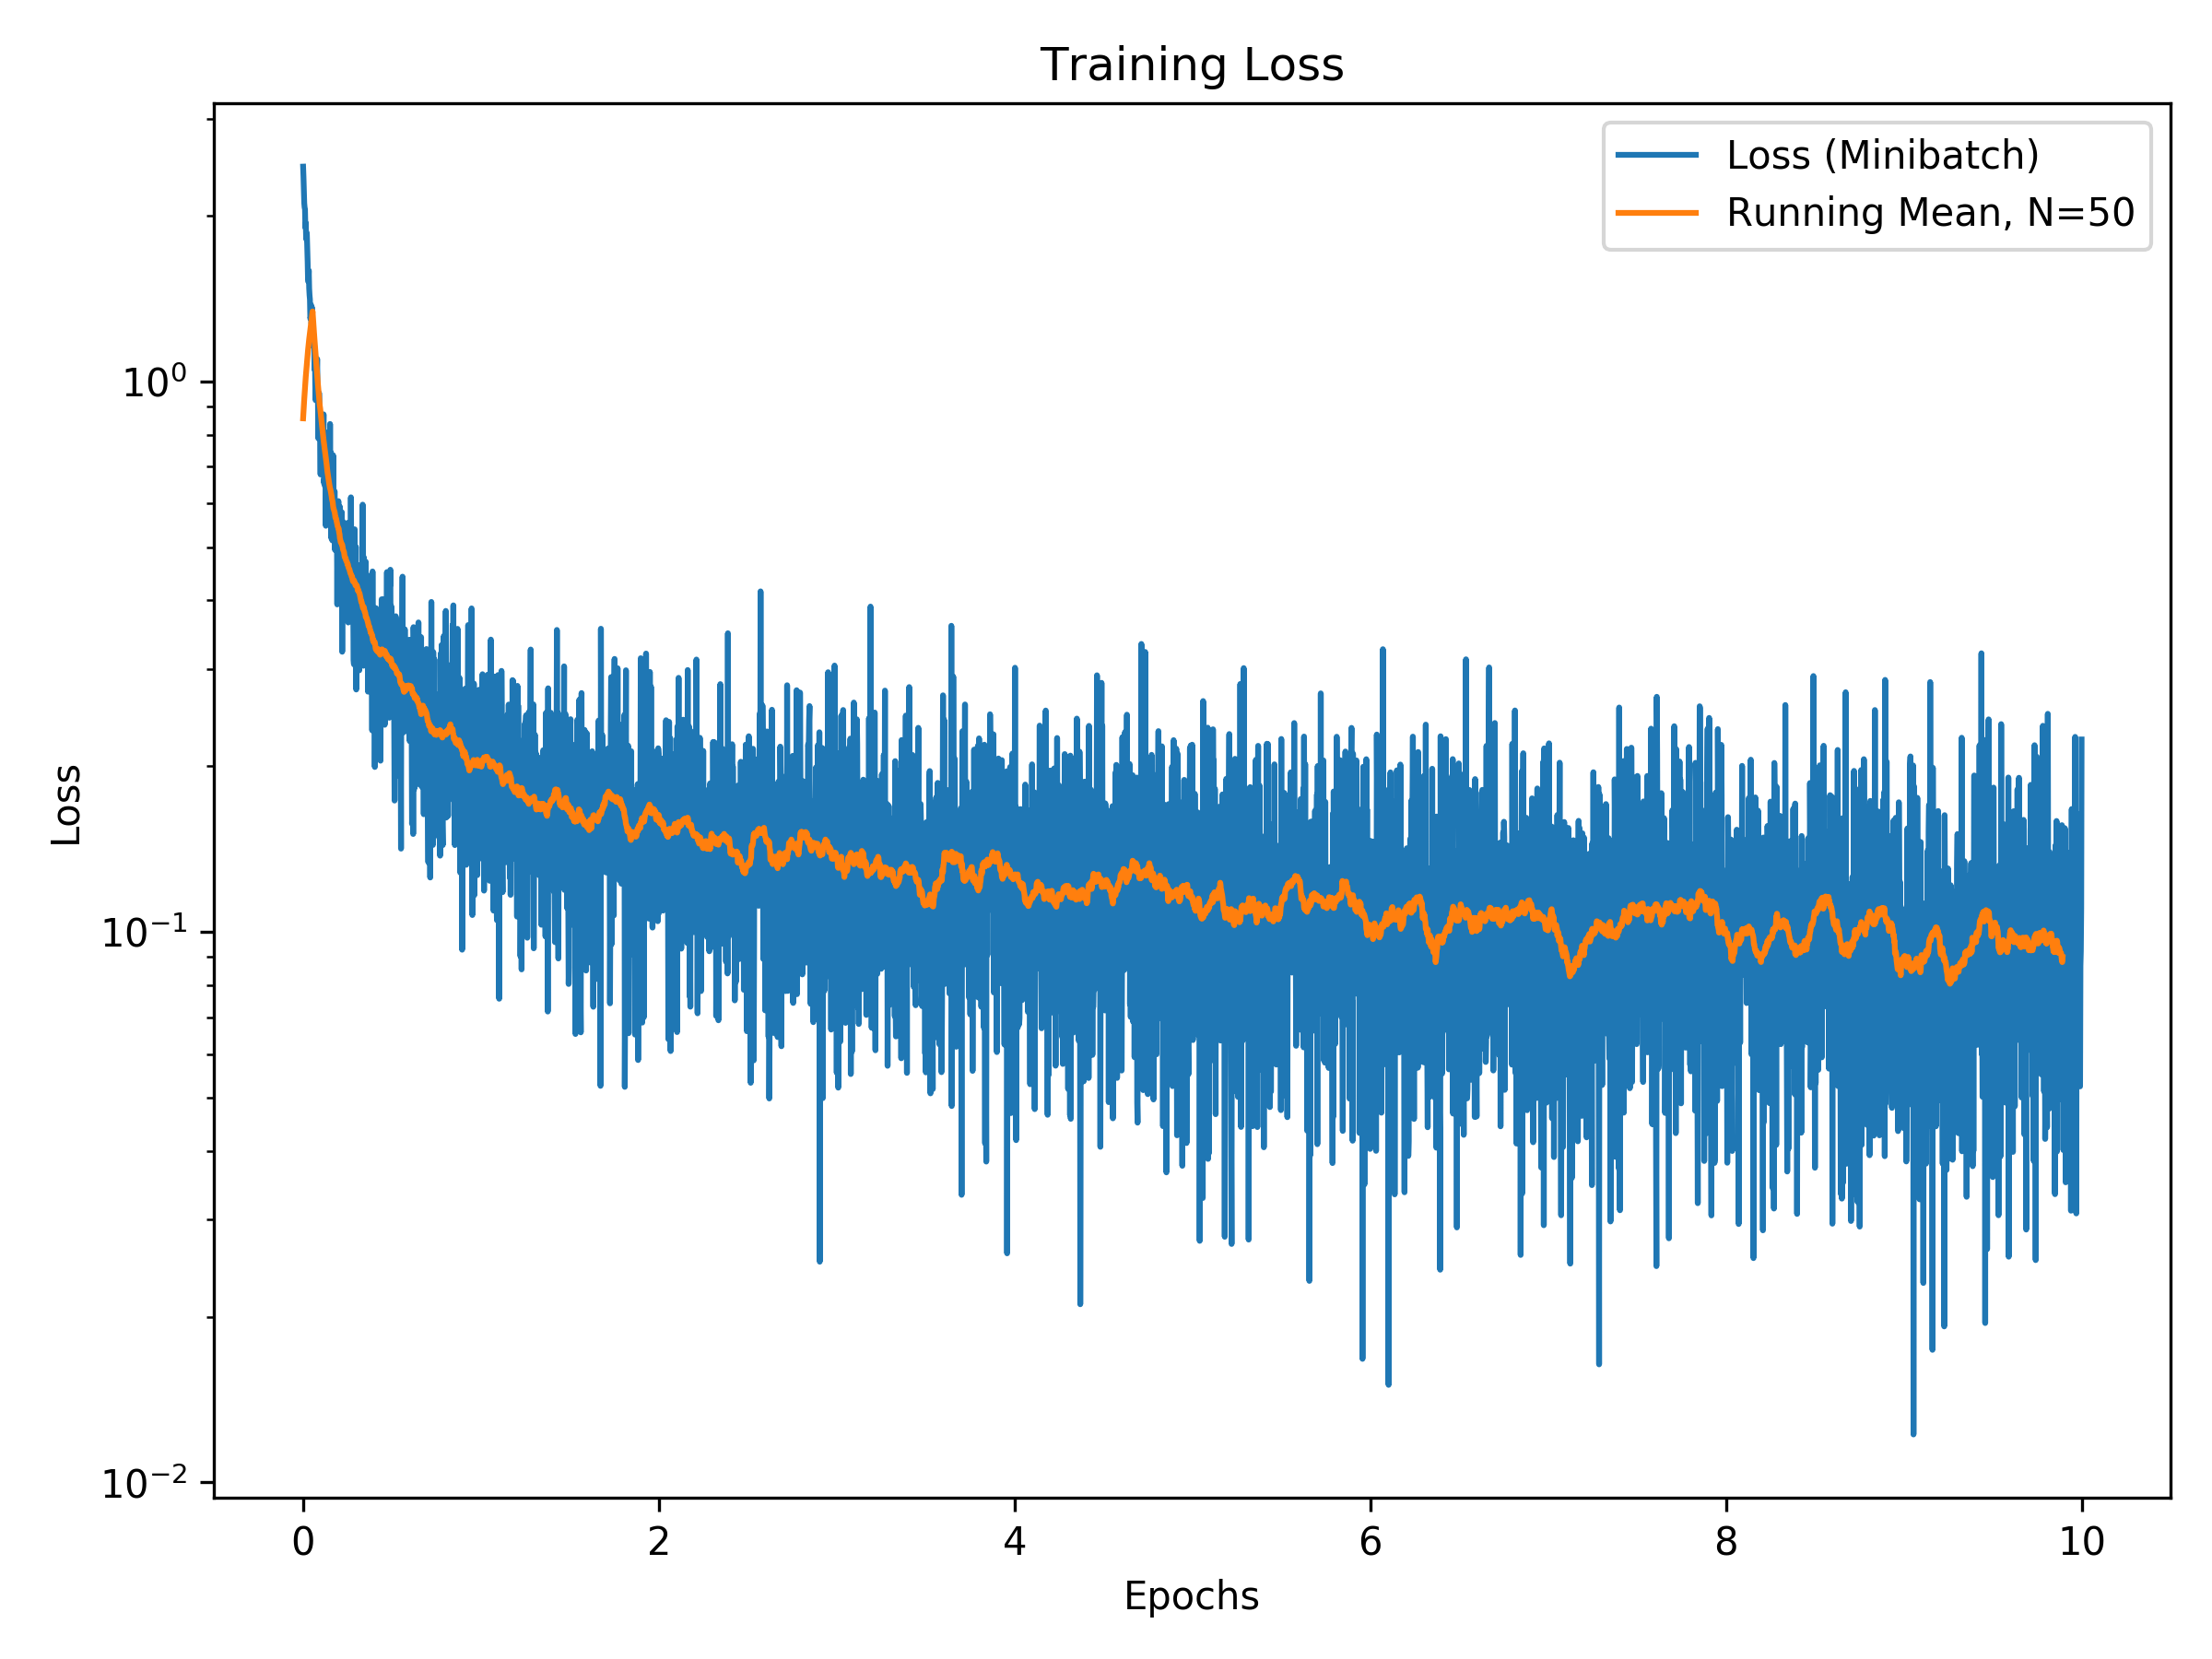
\includegraphics[width=0.8\textwidth]{../../net/images/training_loss}
	\caption{Training Loss}		
	\label{fig:network-train-loss}
\end{subfigure}%
~
\begin{subfigure}[t]{0.5\textwidth}
	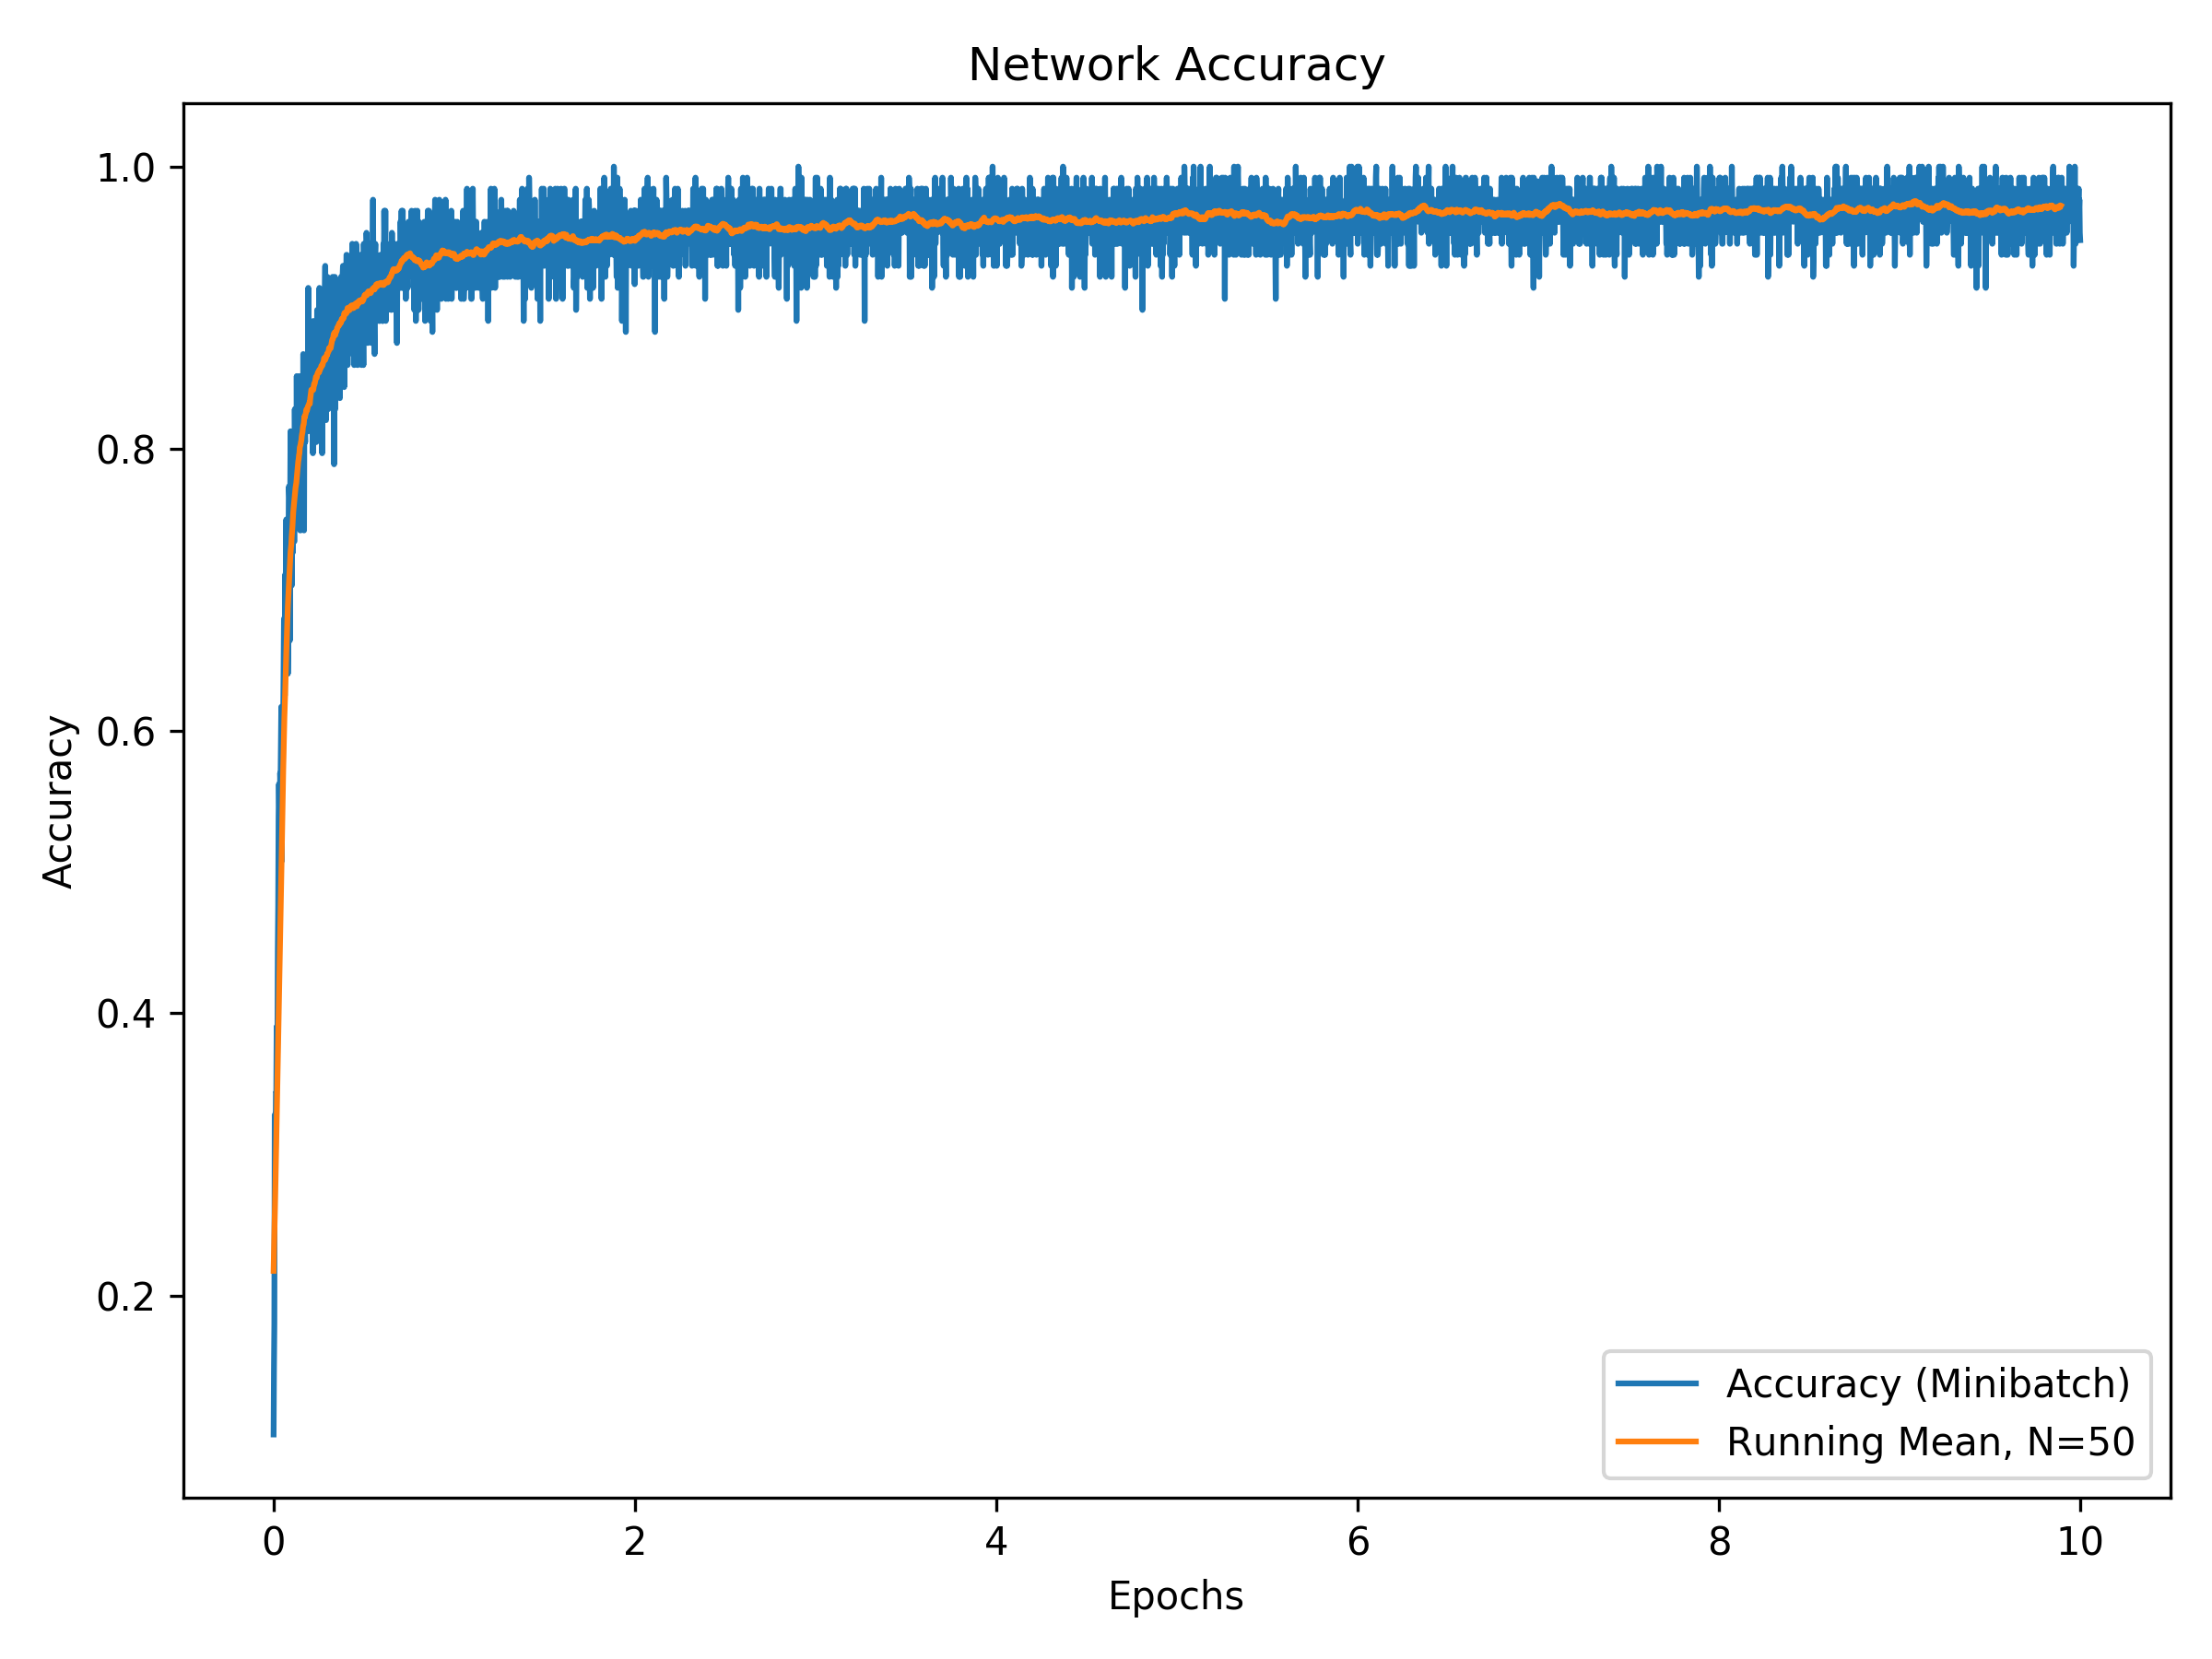
\includegraphics[width=0.8\textwidth]{../../net/images/training_accuracy}
	\caption{Training Accuracy}
	\label{fig:network-train-acc}		
\end{subfigure}
\caption[Network loss and accuracy over the training iterations]{Network loss and accuracy over the training iterations. The blue lines show spikes which occur because of the randomly selected mini batches.}
\label{fig:network-training-graphs}
\end{figure}

\begin{figure}
\centering
\begin{subfigure}[t]{0.5\textwidth}
	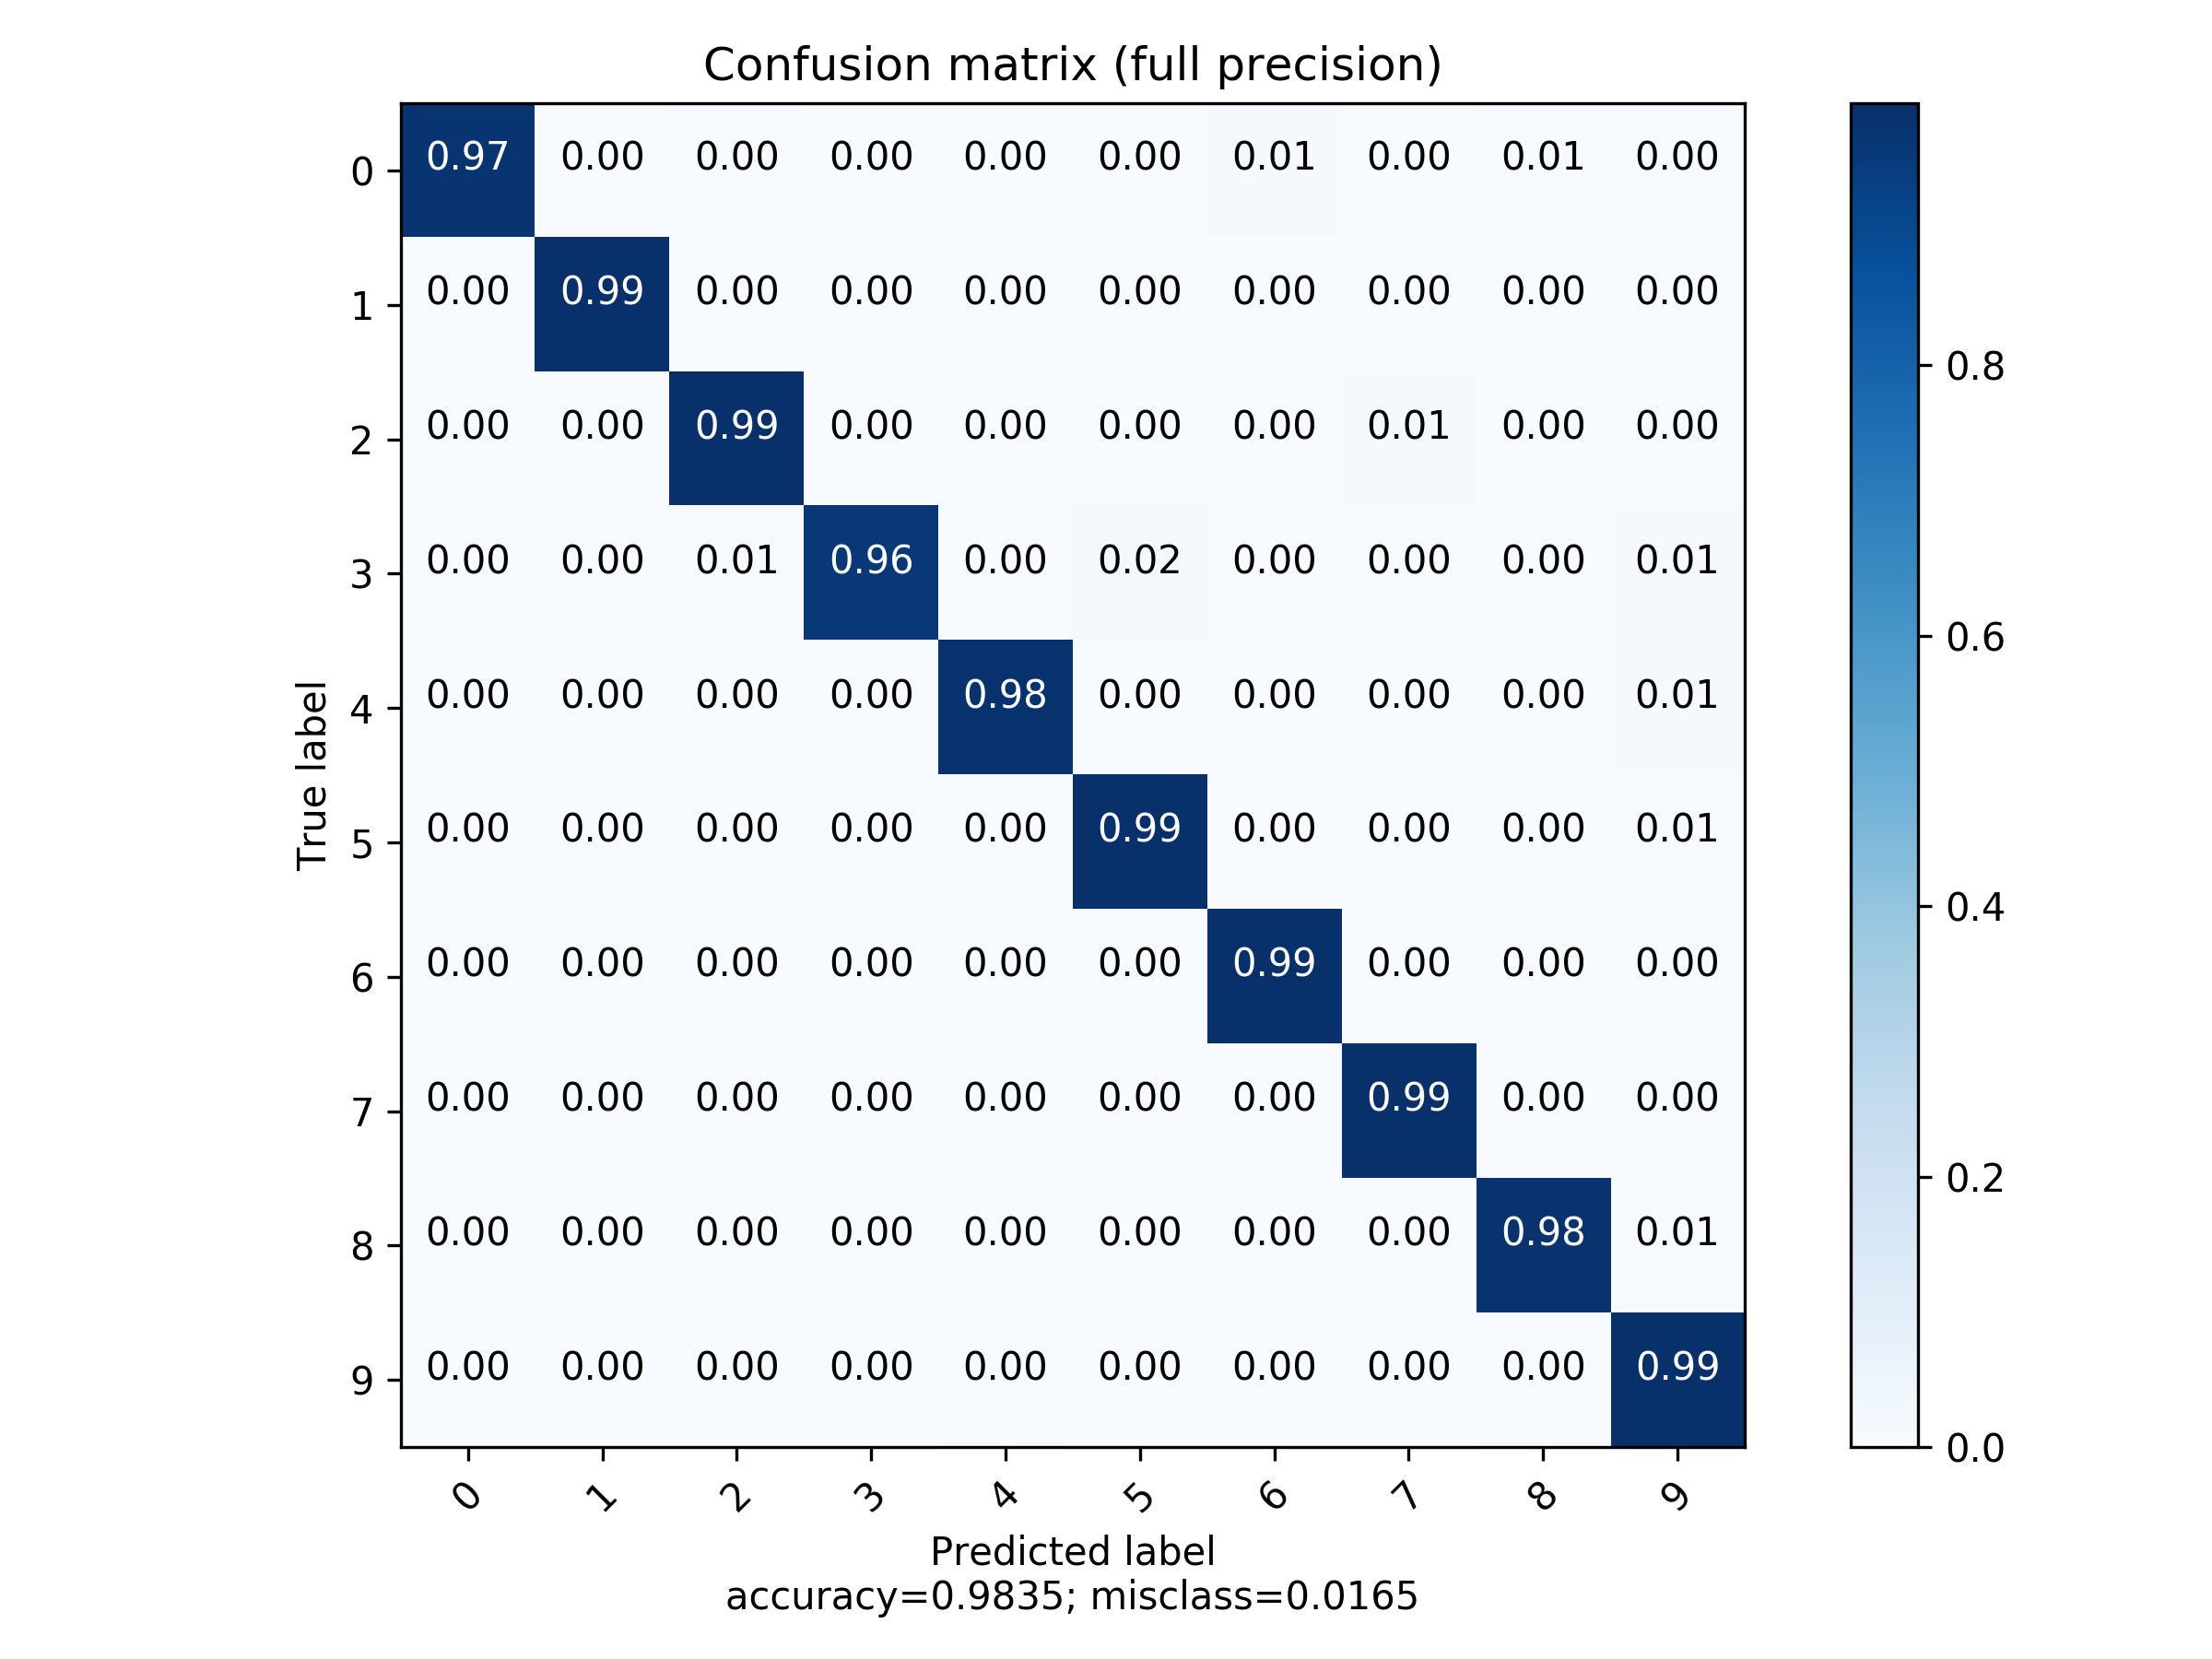
\includegraphics[width=0.9\textwidth]{../../net/images/cm}
	\caption{Floating Point}
	\label{fig:network-test-cm}
\end{subfigure}%
~
\begin{subfigure}[t]{0.5\textwidth}
	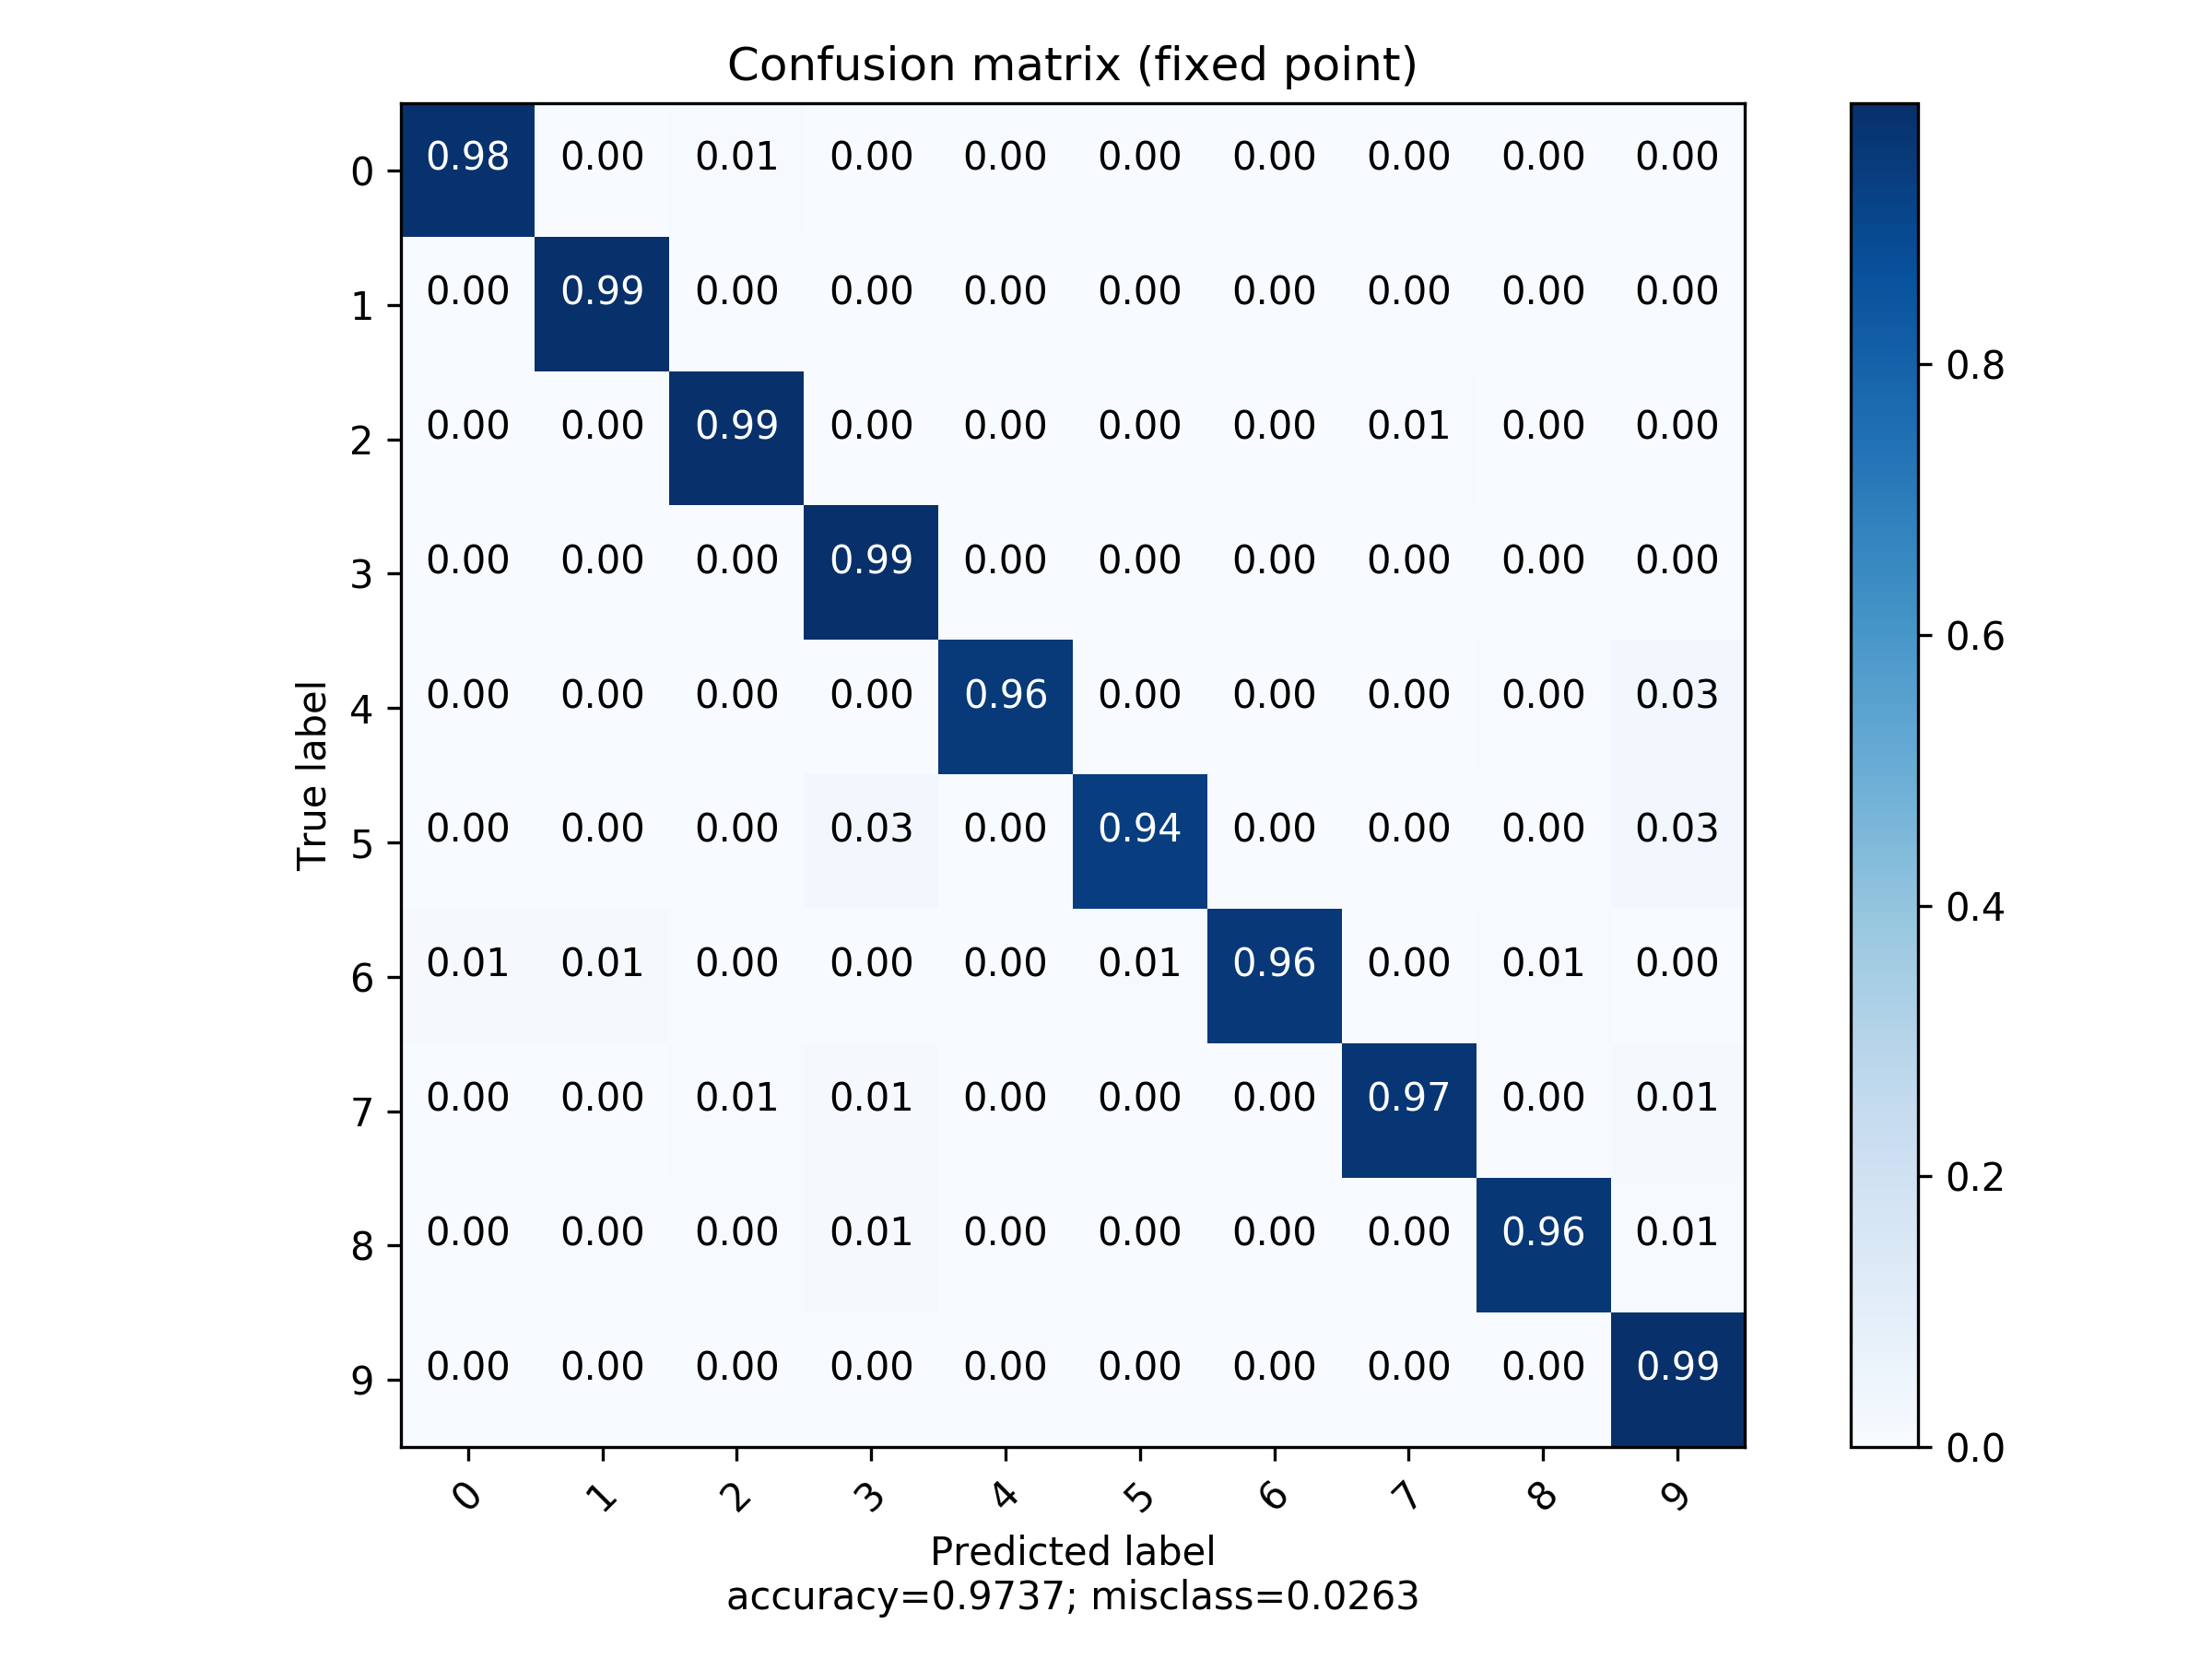
\includegraphics[width=0.9\textwidth]{../../net/images/qcm}
	\caption{Quantized Values}
	\label{fig:network-test-qcm}
\end{subfigure}
\caption{Confusion matrix for the floating point and quantized version of the netowork.}
\label{fig:network-confusion-matrix}
\end{figure}

\section{Quantization}

The network is trained and created using 32bit floating point values in Python. Directly porting this all the weights and biases to the FPGA is due to the limited amount of available resources not feasible. The goal is therefore to reduce the amount of required hardware cells by switching from floating point arithmetic to the less expensive integer arithmetic. Then a floating point value $v$ can be approximately represented as 
\begin{equation}
	v \approx Q \cdot 2 ^{-m}
\end{equation}
where $Q$ and $m$ are integers. In our case all input values of the first layer are guaranteed to lie in the interval $[0,1]$ and all layer weights are known from training. It is therefore possible to precompute the expected range where the output values will be. Depending on this range it is then possible to select a suitable bit width for both $Q$ and $m$.

This is a cost-accuracy trade-off where higher bit widths would improve accuracy as well as increase the amount of hardware resources needed.
In \cite{Wu:2018aa} different strategies of choosing bit widths for $Q$ and $m$ are compared and they observed three main configurations, which are (from simple to advanced):
\begin{enumerate}
	\item Use a $(Q,m)$ configuration for the whole network
	\item Use a $(Q,m)$ configuration for each layer
	\item Use a $(Q,m)$ configuration for each output channel 
\end{enumerate}
In the third configuration the authors could reduce the bit widths the most without sacrificing accuracy this increases the complexity in transferring the weights from layer to layer because the additional shift operations are necessary in order to adjust for the different values of $m$.
In \cite{Wu:2018aa} the authors also deduced from their experiments that the accuracy of the weights can be reduced the most, followed by the activations. By analysing the weights of out network (see Figure~\ref{fig:network-weight-distributions}) a per channel quantization is not necessary, because all weights in a Convolutional Layer are equally distributed among the output channels. Another important property that can be noted is the that the weights do have zero mean and most of the values lie very close to zero. Because of the usage of ReLU layer the situation is different for the activations where unsigned integers can be used, the distributions are shown in Figure~\ref{fig:network-activations-distributions}.

Using the distribution histograms we then defined derived the necessary bitwidths for $Q$ and $m$. In our experiments we were able to reduce them to \SI{8}{\bit}, if we used a single configuration for the whole network and also reducing them down to 4bit if the bitwidth configuration is selected for each layer independently with an accuracy drop from around \SI{98.35}{\percent} to \SI{97.37}{\percent}. The strategy to the select the values for $(Q,m)$ was
\begin{enumerate}
	\item Find the value range of the weights and output activations of each layer
	\item Select suitable $(Q,m)$ values that most activations fall in that range
	\item Calculate the bit widths and exponents of the multiplication operation
	\item Add $\lceil \log_2(n) \rceil$ extra bits to account for the accumulation of $n$ values
	\item Compare the accumulated exponents and with the exponents of the successive layers input exponents. The difference is the amount of shift required
\end{enumerate}
It is noteworthy that the values for $m$ do not need to be stored in the final network, because those are only used to determine the amount of shifts between the layers. Also the values need to be clipped to their maximum and minimum values. The complete configuration of the network is summarized in Table~\ref{tab:quantization-linear-params}.

Ad 4 and 5: The transition from a layer to the next often changes the exponent $m$ and the available bitwidth. To account for this the values need to accordingly shifted. Also the decreased bitwidth needs clipping.

For our network only linear quantization has been used but also non-linear quantization, e.g. in a $\log_2$ way which is proposed in \cite{Lee:2017aa}. Experiments showed that using this technique even further down to \SI{3}{\bit} weights in our case.
Another optimization technique that could be explored is the systematically removing of weights (connections) of the network and reduce the amount of operations needed to be performed, a process refered to as ''pruning'' \cite{Zhu:2017aa}. This was not explicitly performed but is implicitly done by low bit quantization.

\begin{table}[hbt]
  \centering
  \begin{tabular}{lcccc}
	\toprule
    Network Part 	  & $|Q|$ & $m$ & $\pm$ & $v$ (real value range) \\
	\midrule
    Input 		 	  &  8    & 8  & $+$   & $[0,1]  $ \\
    L1: Weights 	  &  4    & 2  & $\pm$ & $[-2,2] $ \\
    L1: Intermediates & 12    & 10 & $\pm$ & $[-2,2] $ \\
    L1: Accumulated   & 16    & 10 & $\pm$ & 		   \\
    \midrule
    L1 $\to$ L2 	  & \multicolumn{4}{c}{Rshift by $10-2$ and clip values in range $[0,15]$} \\
    \midrule
    L2: Input 		  &  4    & 2  & $+$   & $[-2,2] $ 	   \\
    L2: Weights 	  &  4    & 5  & $\pm$ & $[-0.5,0.5] $ \\
    L2: Intermediates &  8    & 7  & $\pm$ & $[-1,1] $ \\
    L2: Accumulated   & 16    & 7  & $\pm$ &  			   \\
    \midrule
    L2 $\to$ L3 	  & \multicolumn{4}{c}{Rshift by $7-0$ and clip values in range $[0,15]$} \\
    \midrule
    L3: Input 		  &  4    & 0  & $+$   & $[0,15] $     \\
    L3: Weights 	  &  4    & 5  & $\pm$ & $[-0.5,0.5] $ \\
    L3: Intermediates &  8    & 5  & $\pm$ & $[-7.5,7.5] $ \\
    L3: Accumulated   & 19    & 5  & $\pm$ &               \\
    \midrule
    L3 $\to$ L4 	  & \multicolumn{4}{c}{Rshift by $5-0$ and clip values in range $[0,15]$} \\
    \midrule
    L4: Input 		  &  4    & 0  & $+$   & $[0,15] $ \\
    L4: Weights 	  &  4    & 5  & $\pm$ & $[-0.5,0.5] $ \\
    L4: Intermediates &  8    & 5  & $\pm$ & $[-7.5,7.5] $ \\
    L4: Accumulated   & 14    & 5  & $\pm$ & $[0,1] $ \\
    \bottomrule
  \end{tabular}
  \caption[Quantization parameters for the 4bit network]{Quantization parameters for the 4bit network. The intermediate terms are the values after the multiplication operation and the accumulated term denotes values after summing up of weighted inputs including bias in a channel.}
  \label{tab:quantization-linear-params}
\end{table}


%% WEIGHT DISTTRIBUTIONS
\begin{figure}[htbp]
    \centering
    \begin{subfigure}[t]{0.5\textwidth}
        \centering
        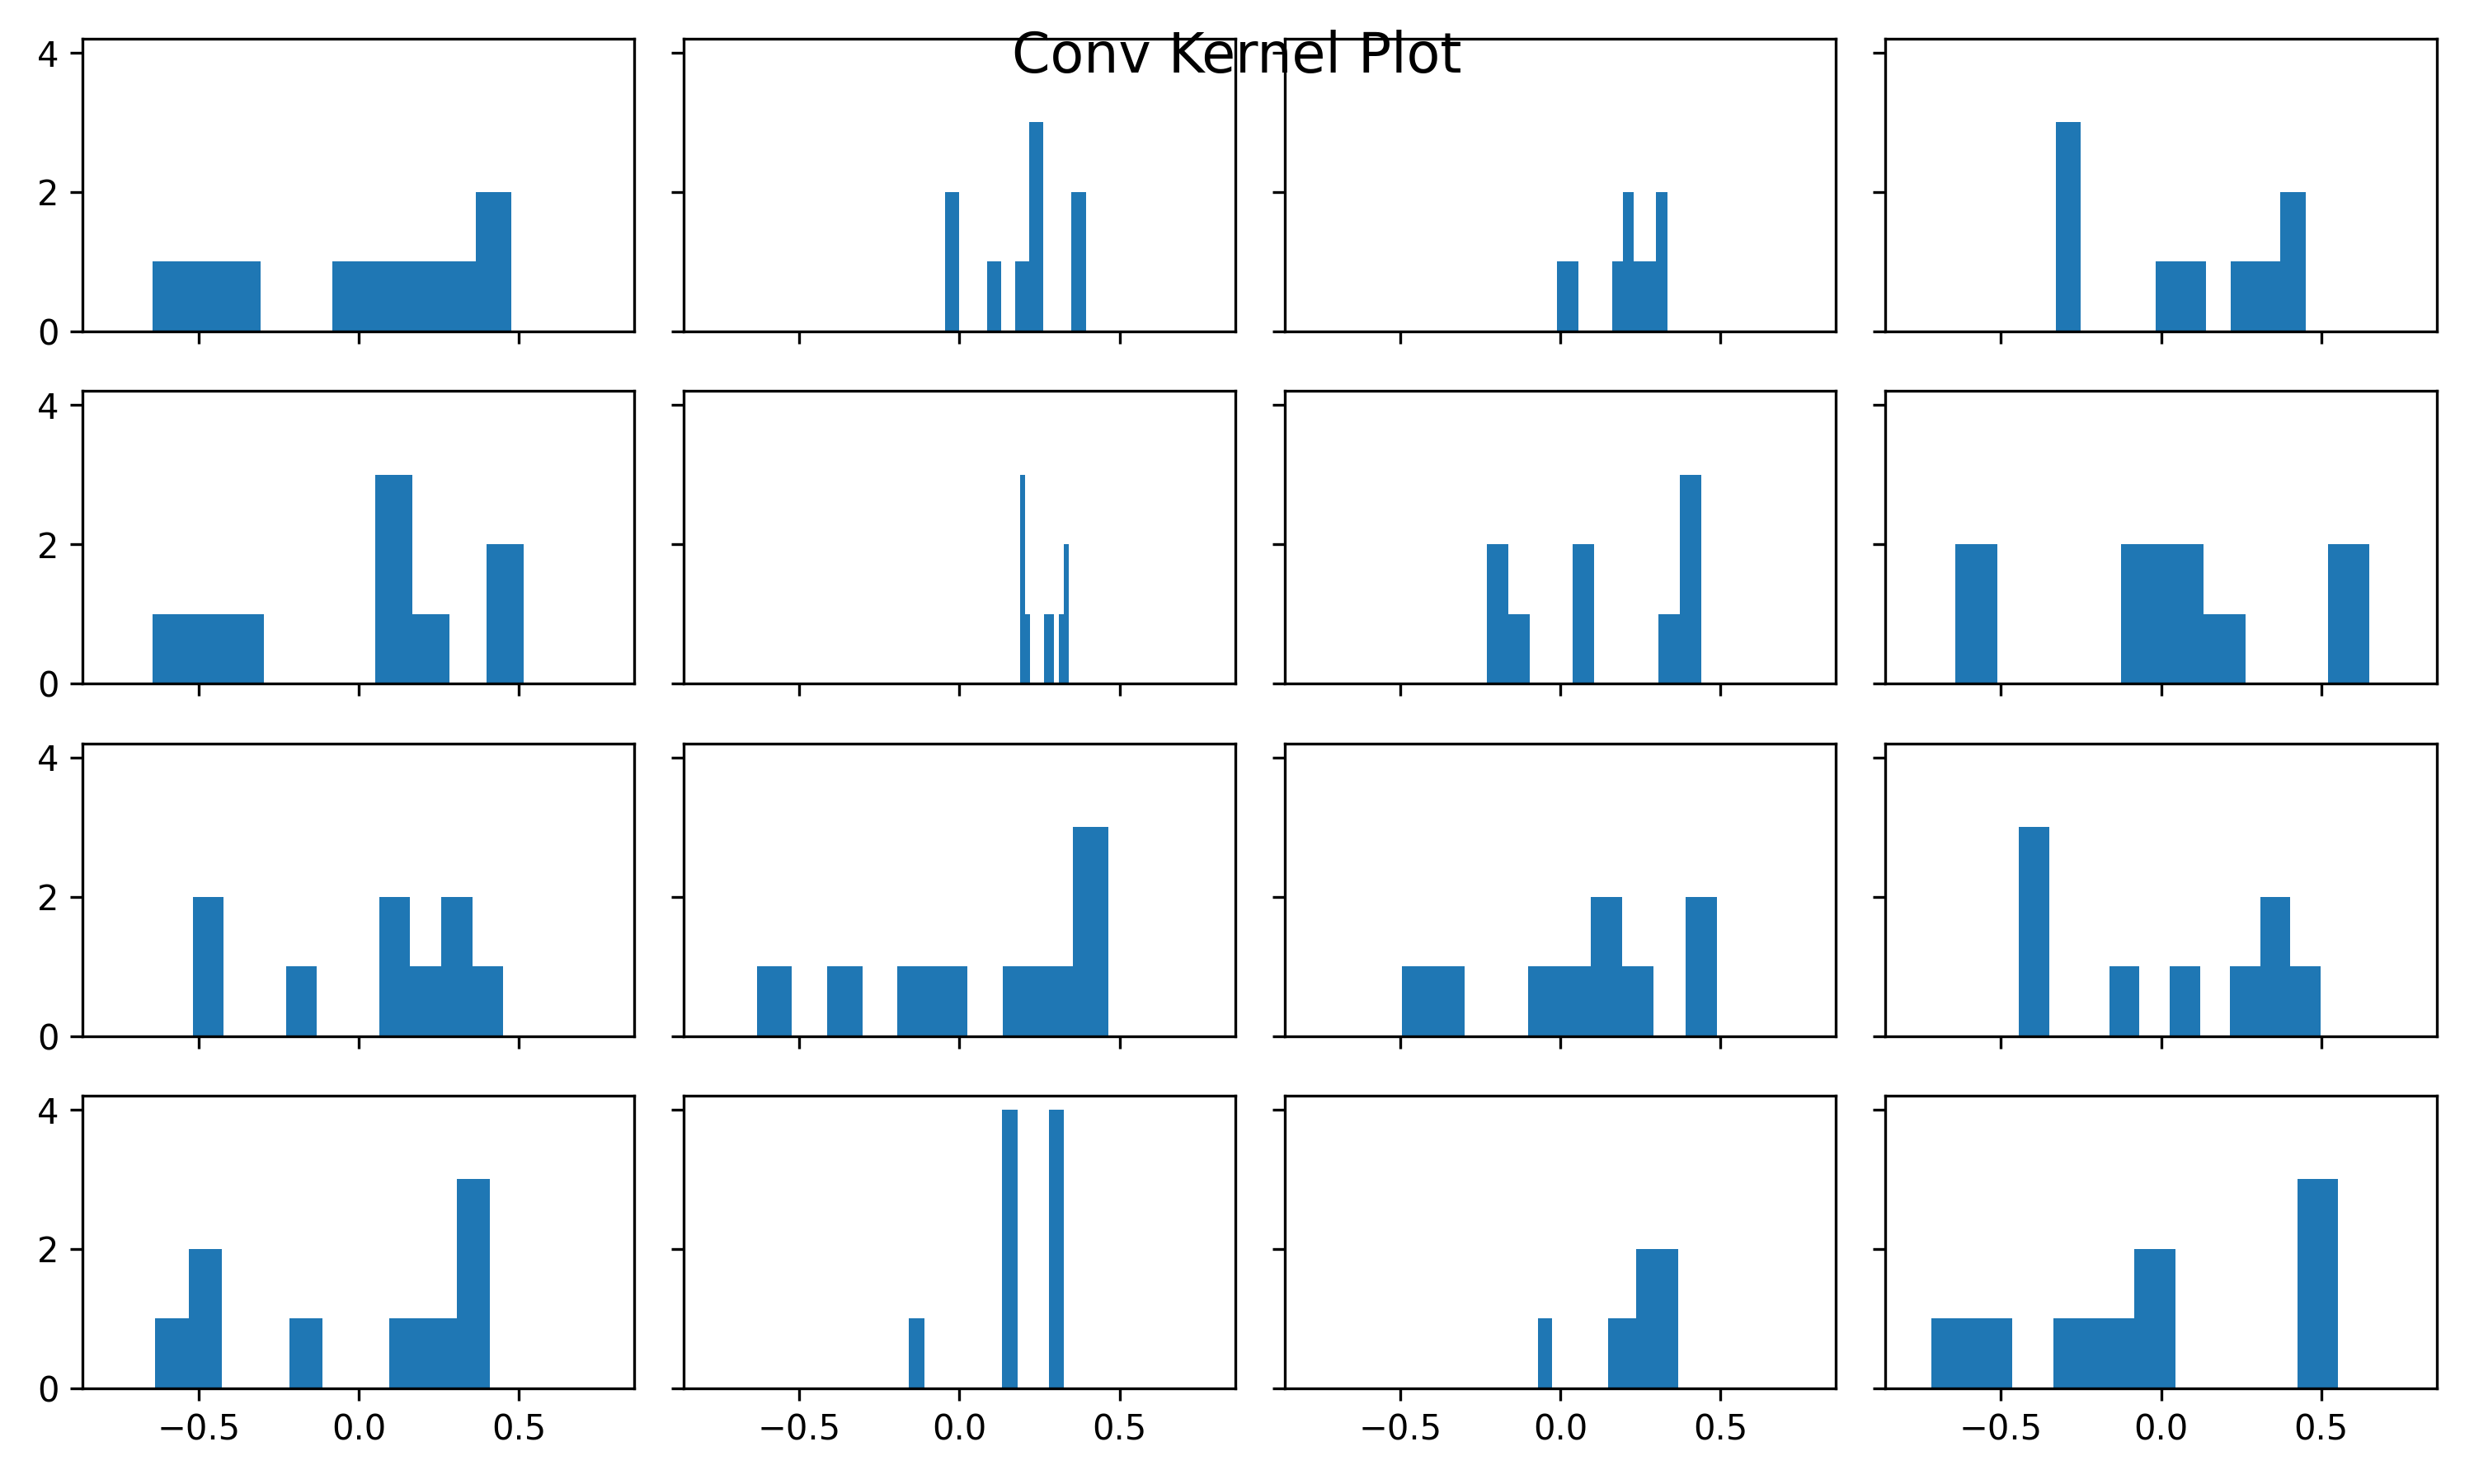
\includegraphics[height=1.6in]{../../net/images/hist_cn1_k}
        \caption{Convolutional Layer 1}
    \end{subfigure}%
    ~ 
    \begin{subfigure}[t]{0.5\textwidth}
        \centering
         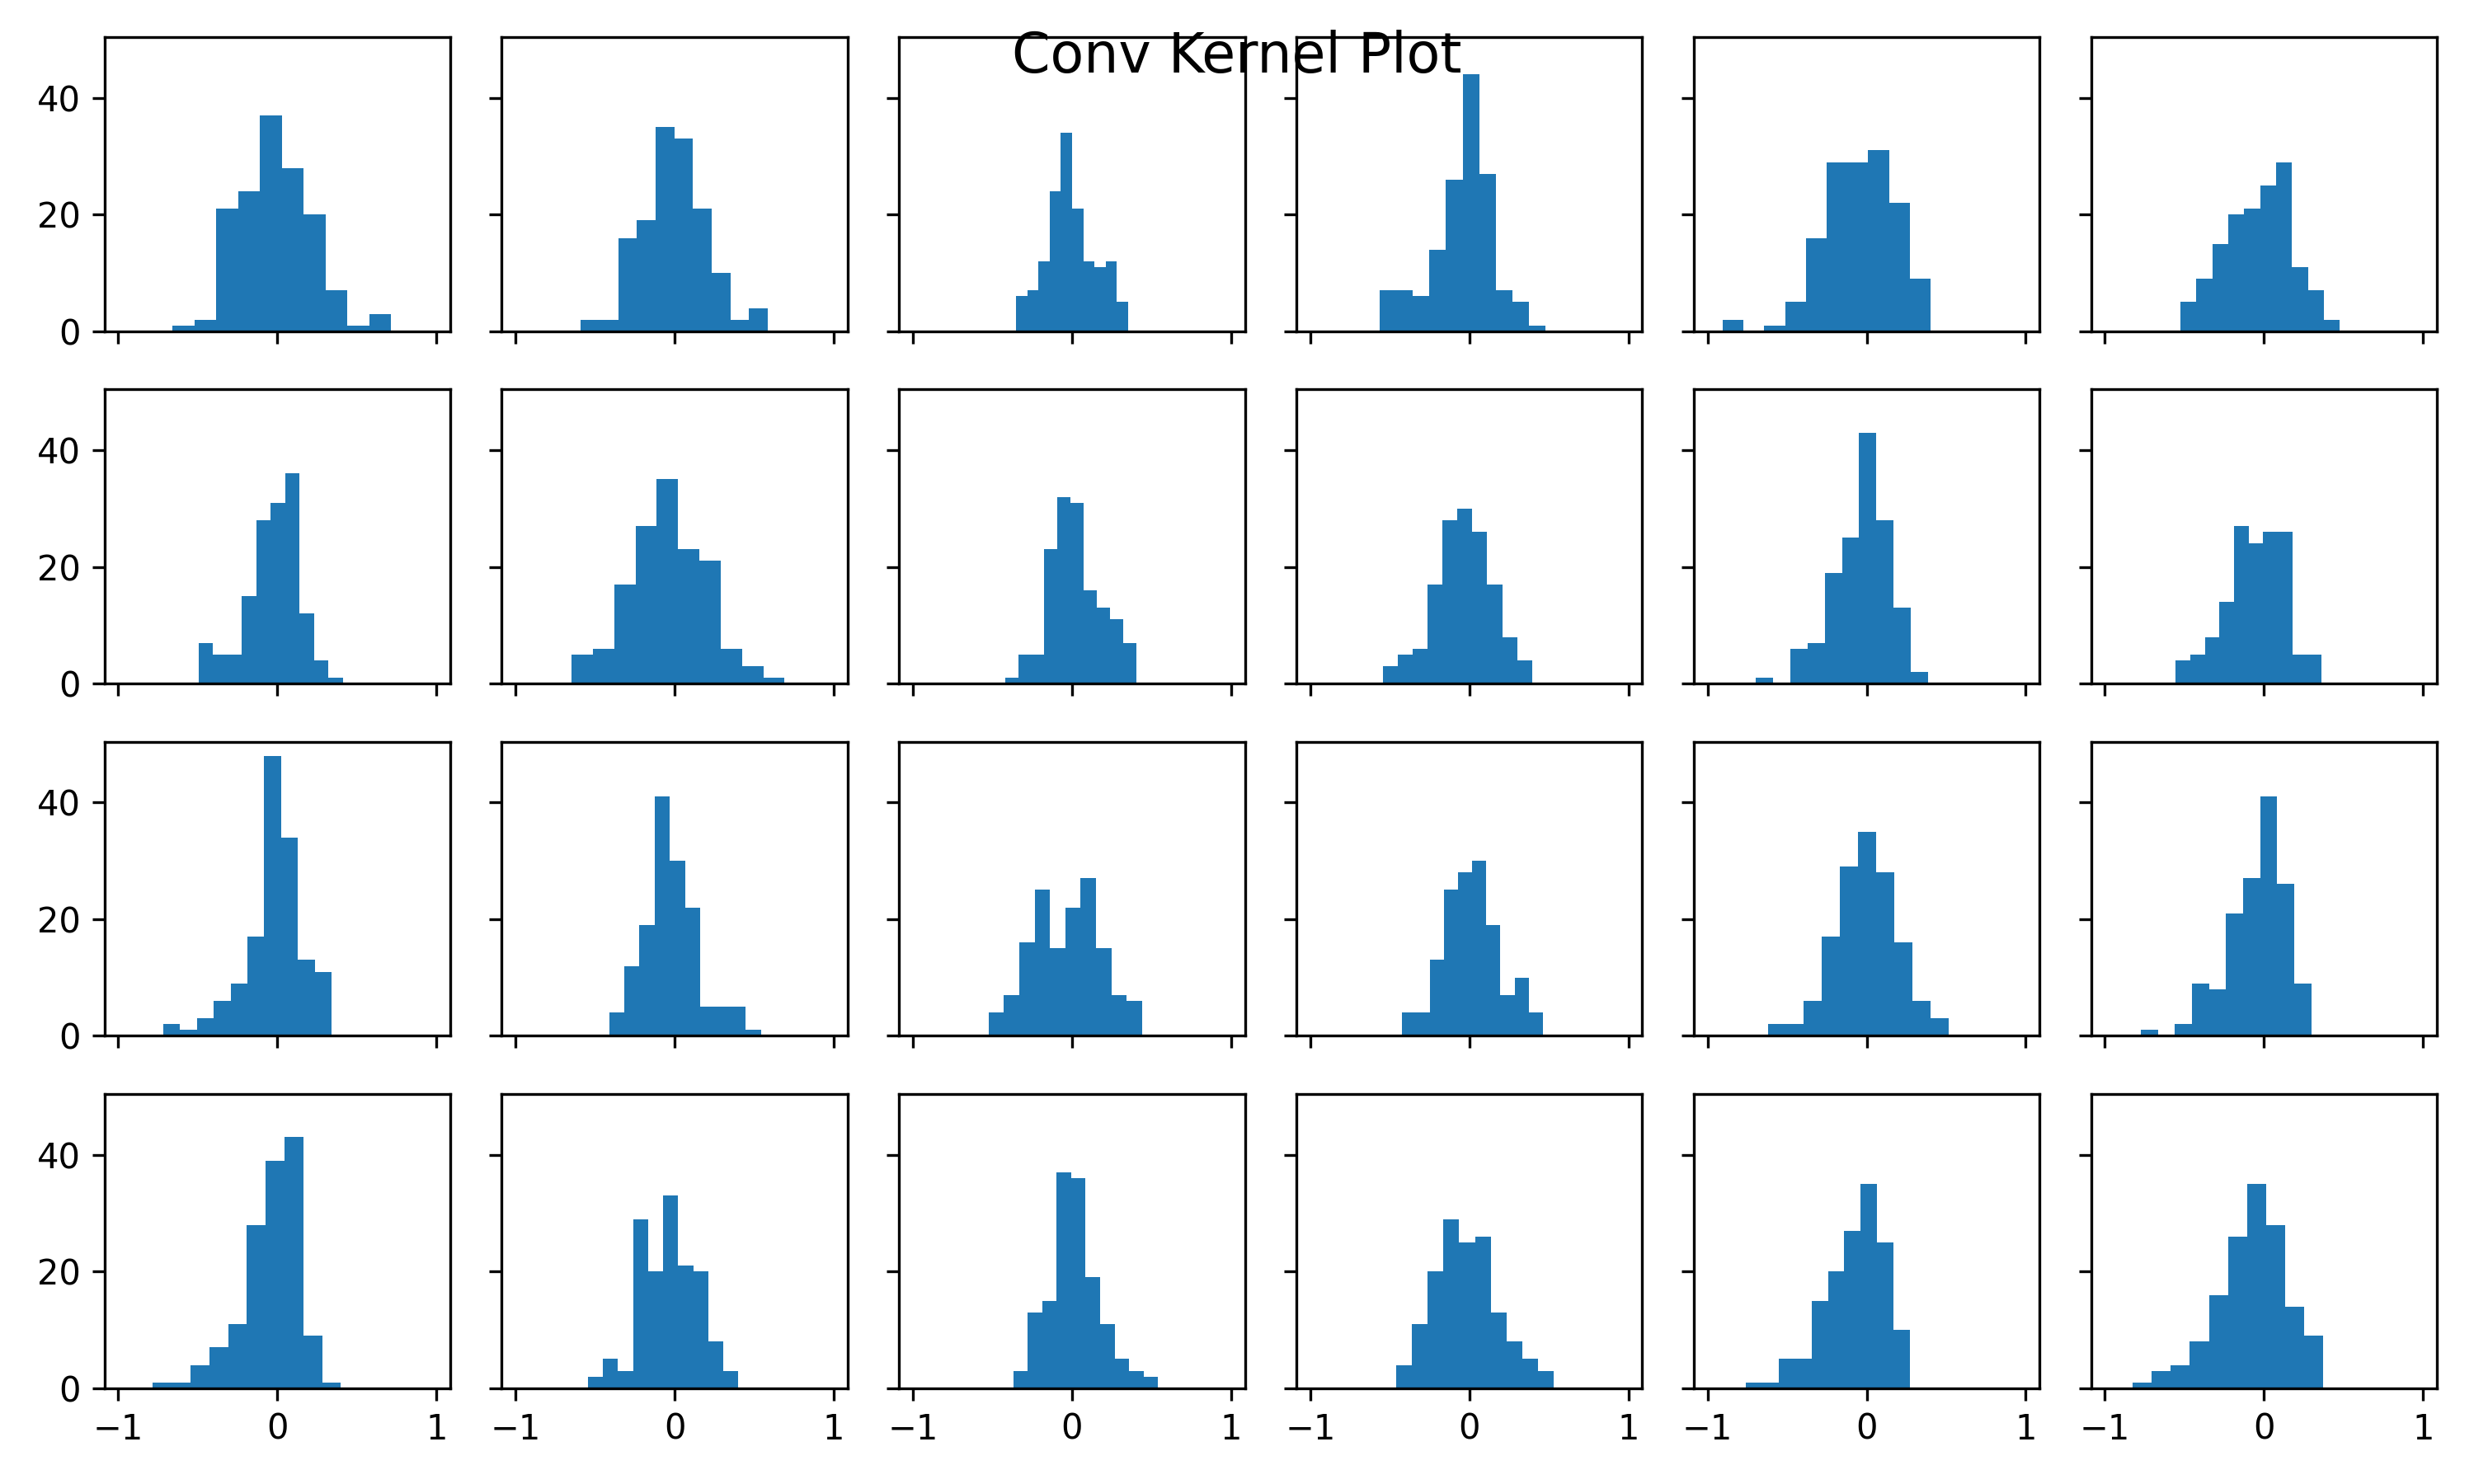
\includegraphics[height=1.6in]{../../net/images/hist_cn2_k}
        \caption{Convolutional Layer 2}
    \end{subfigure}%
    \\
    \begin{subfigure}[t]{0.5\textwidth}
        \centering
        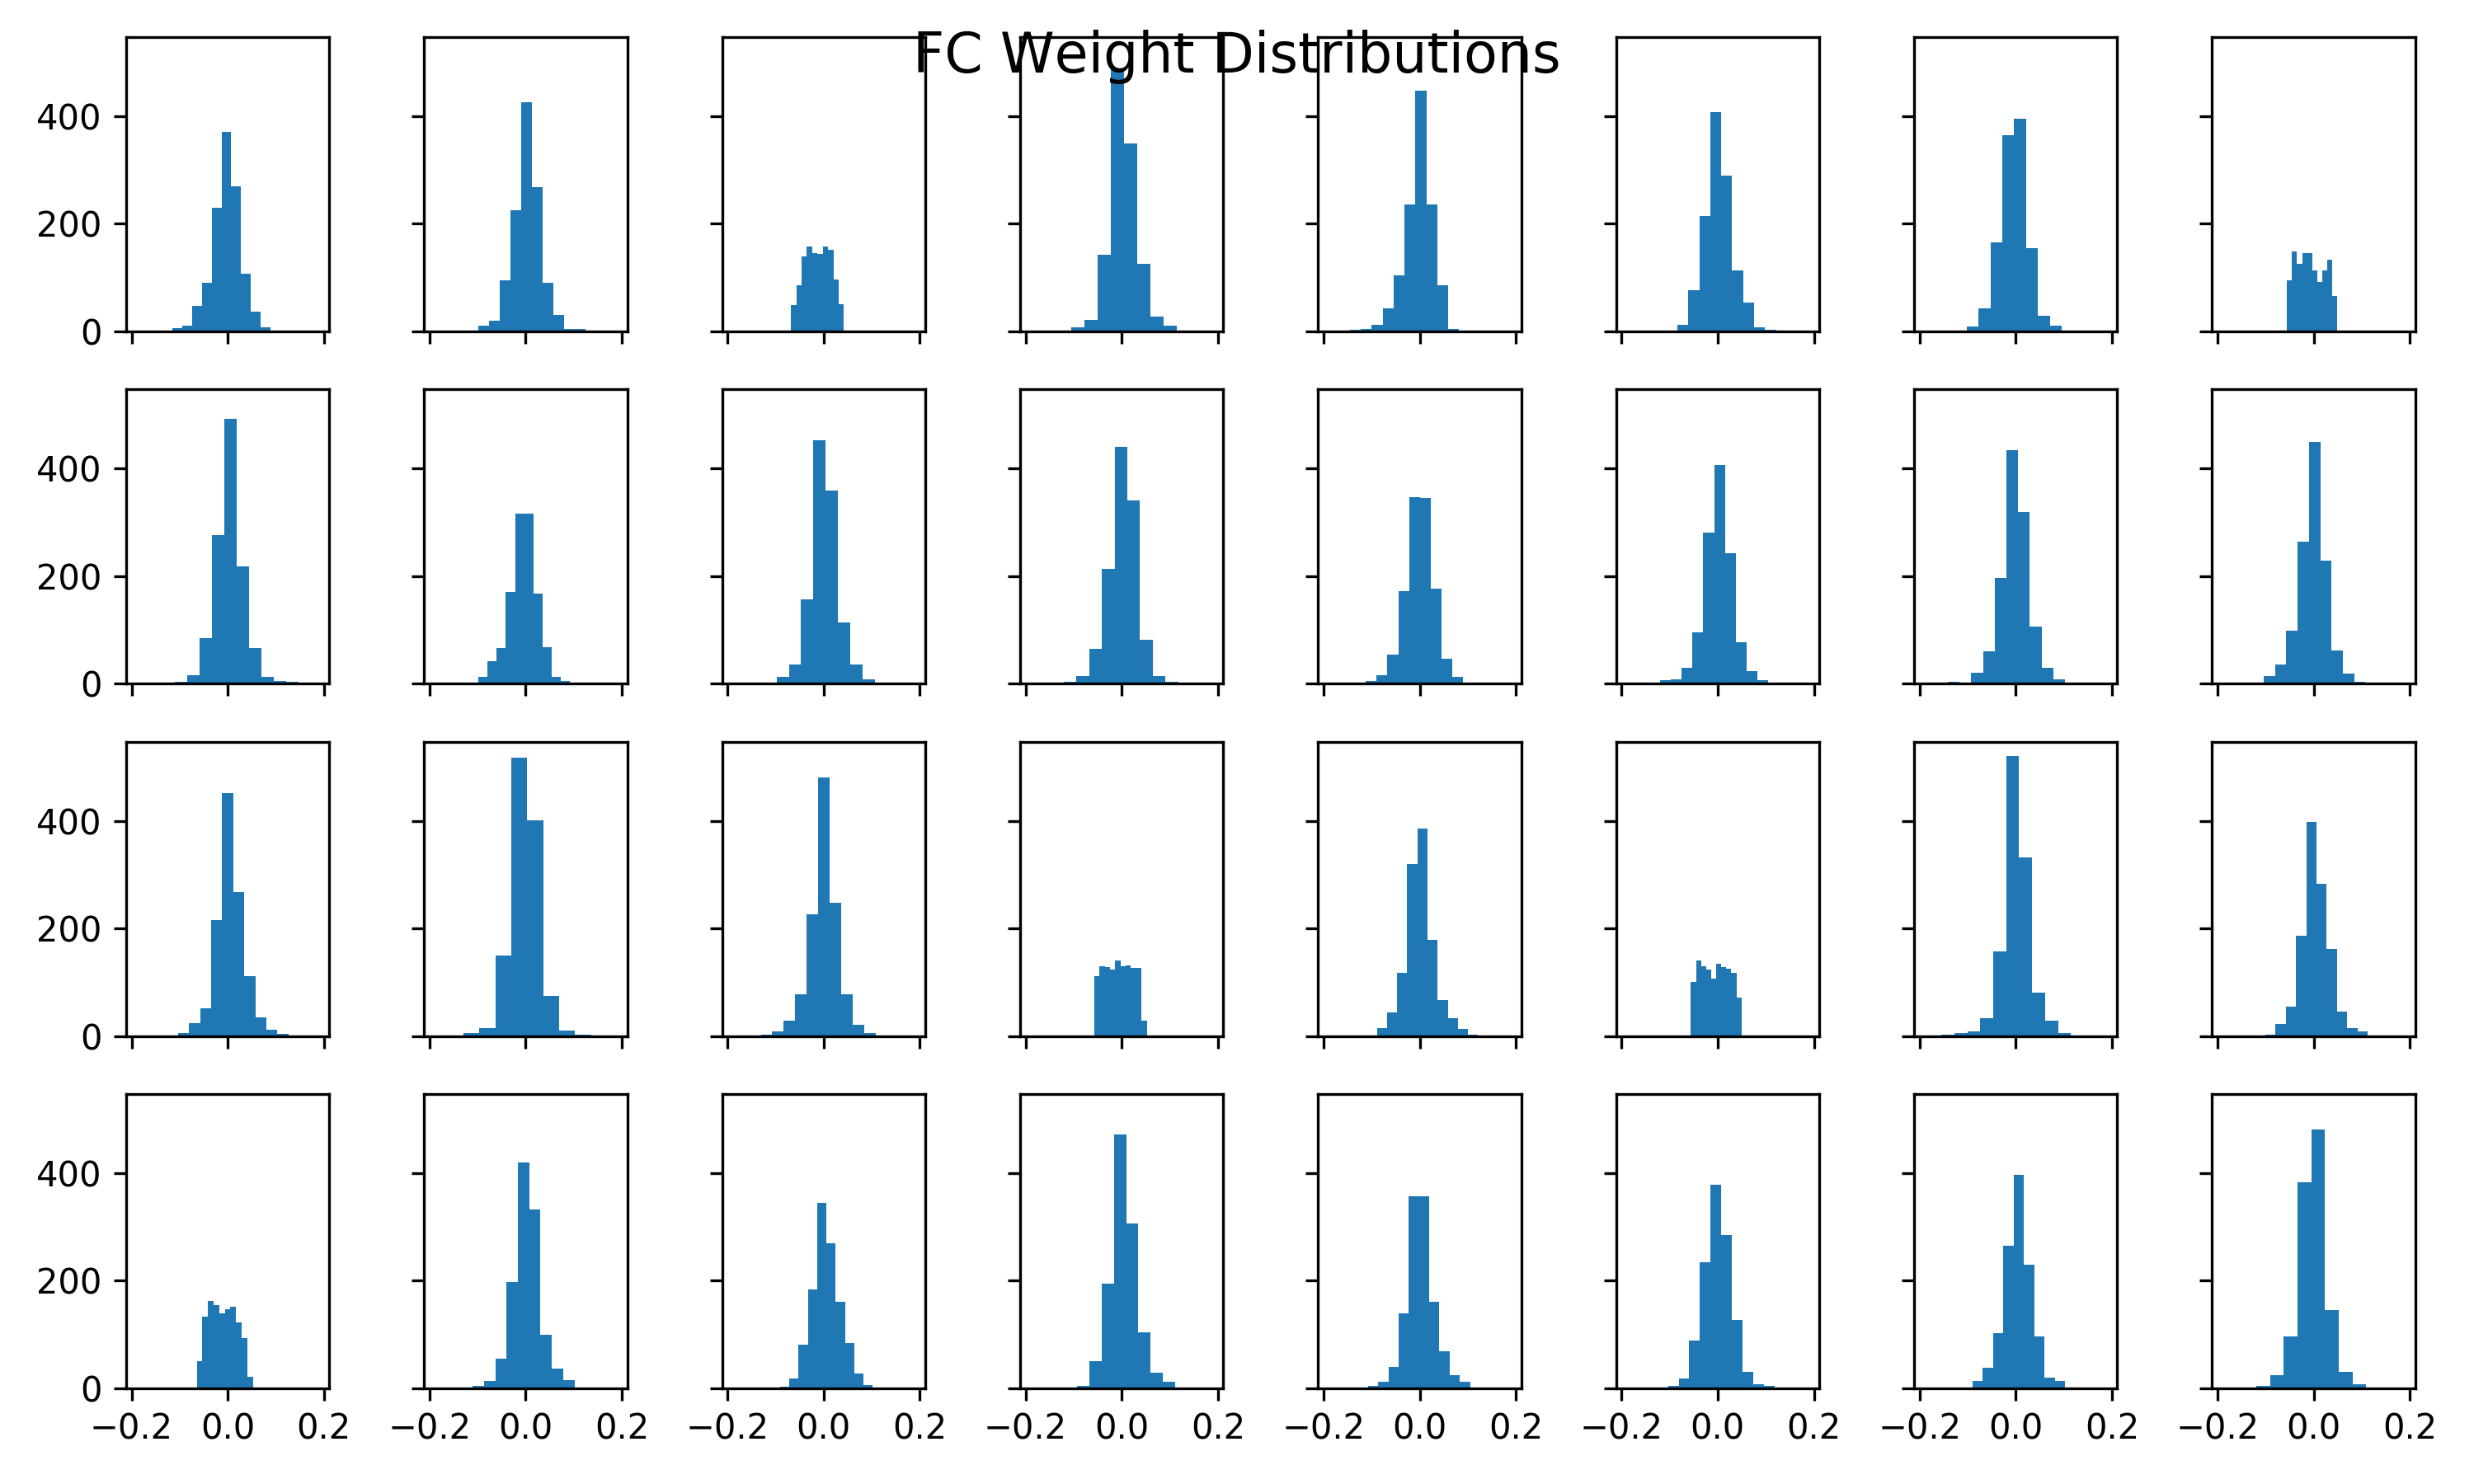
\includegraphics[height=1.6in]{../../net/images/hist_fc1_w}
        \caption{Fully Connected Layer 1}
    \end{subfigure}%
    ~ 
    \begin{subfigure}[t]{0.5\textwidth}
        \centering
         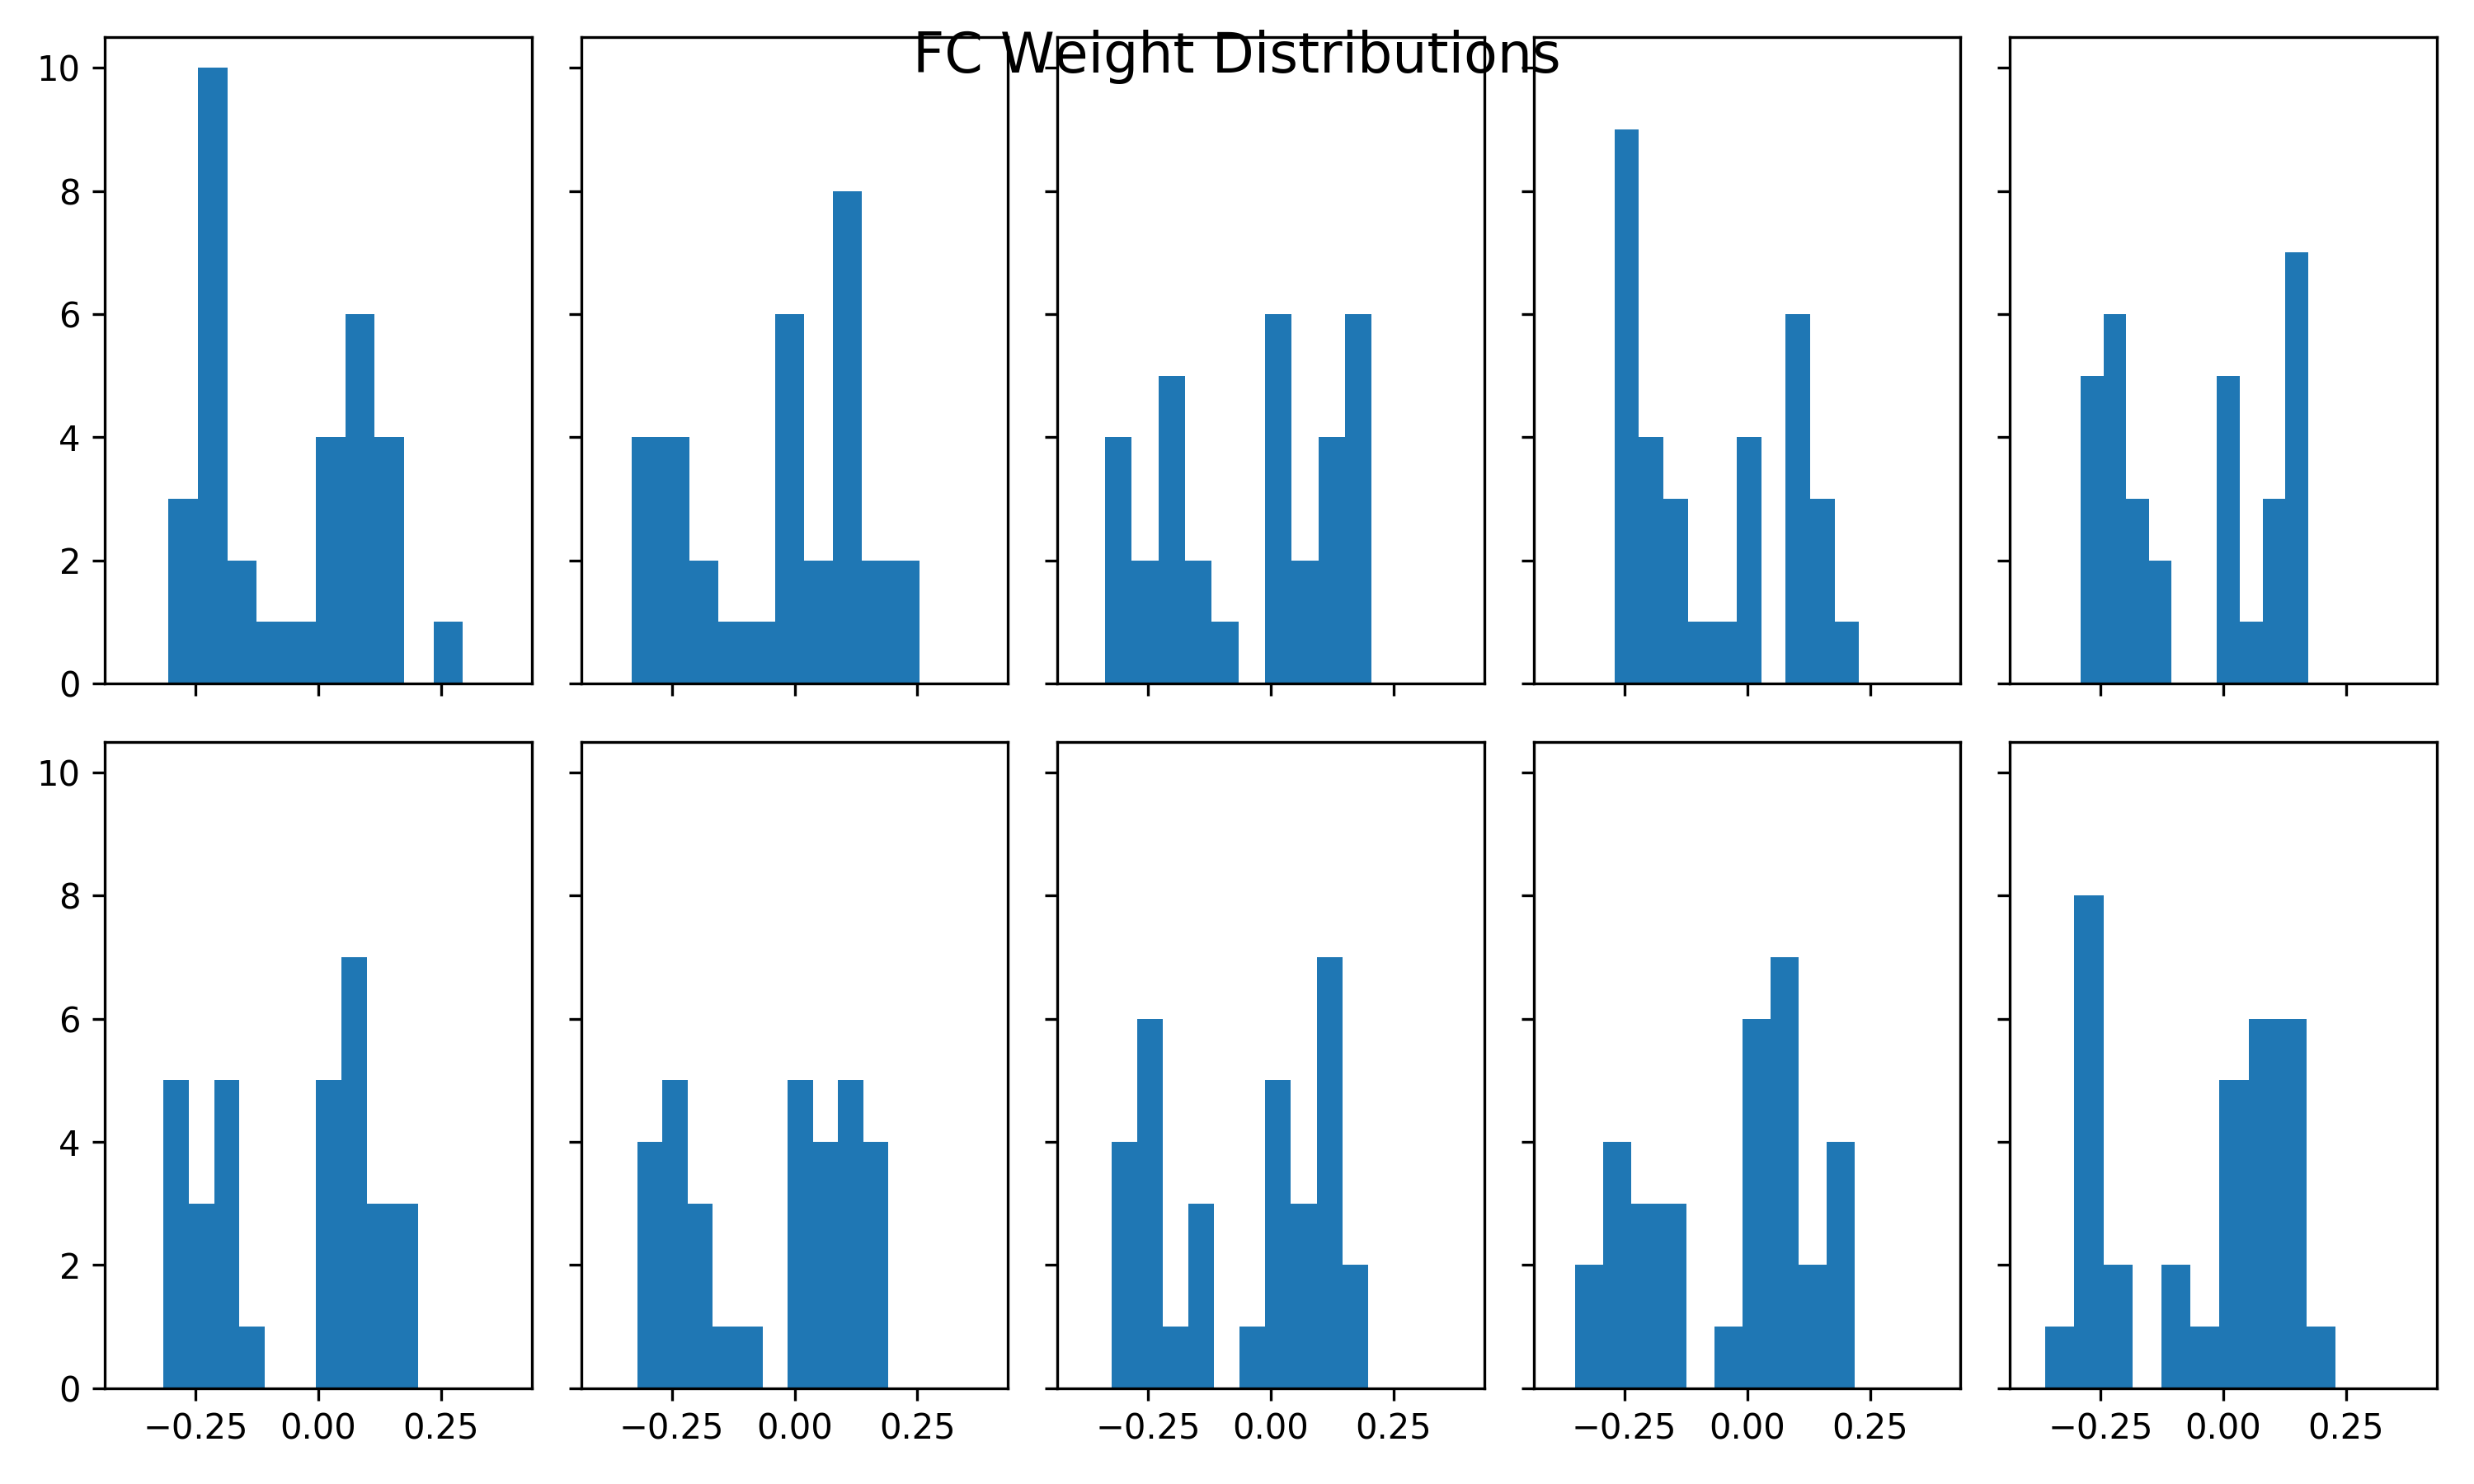
\includegraphics[height=1.6in]{../../net/images/hist_fc2_w}
        \caption{Fully Connected Layer 2}
    \end{subfigure}
    \caption{Distribution of the network weights for the different layers}
    \label{fig:network-weight-distributions}
\end{figure}


%% ACTIVATIONS DISTTRIBUTIONS
\begin{figure}[htbp]
    \centering
    \begin{subfigure}[t]{0.5\textwidth}
        \centering
        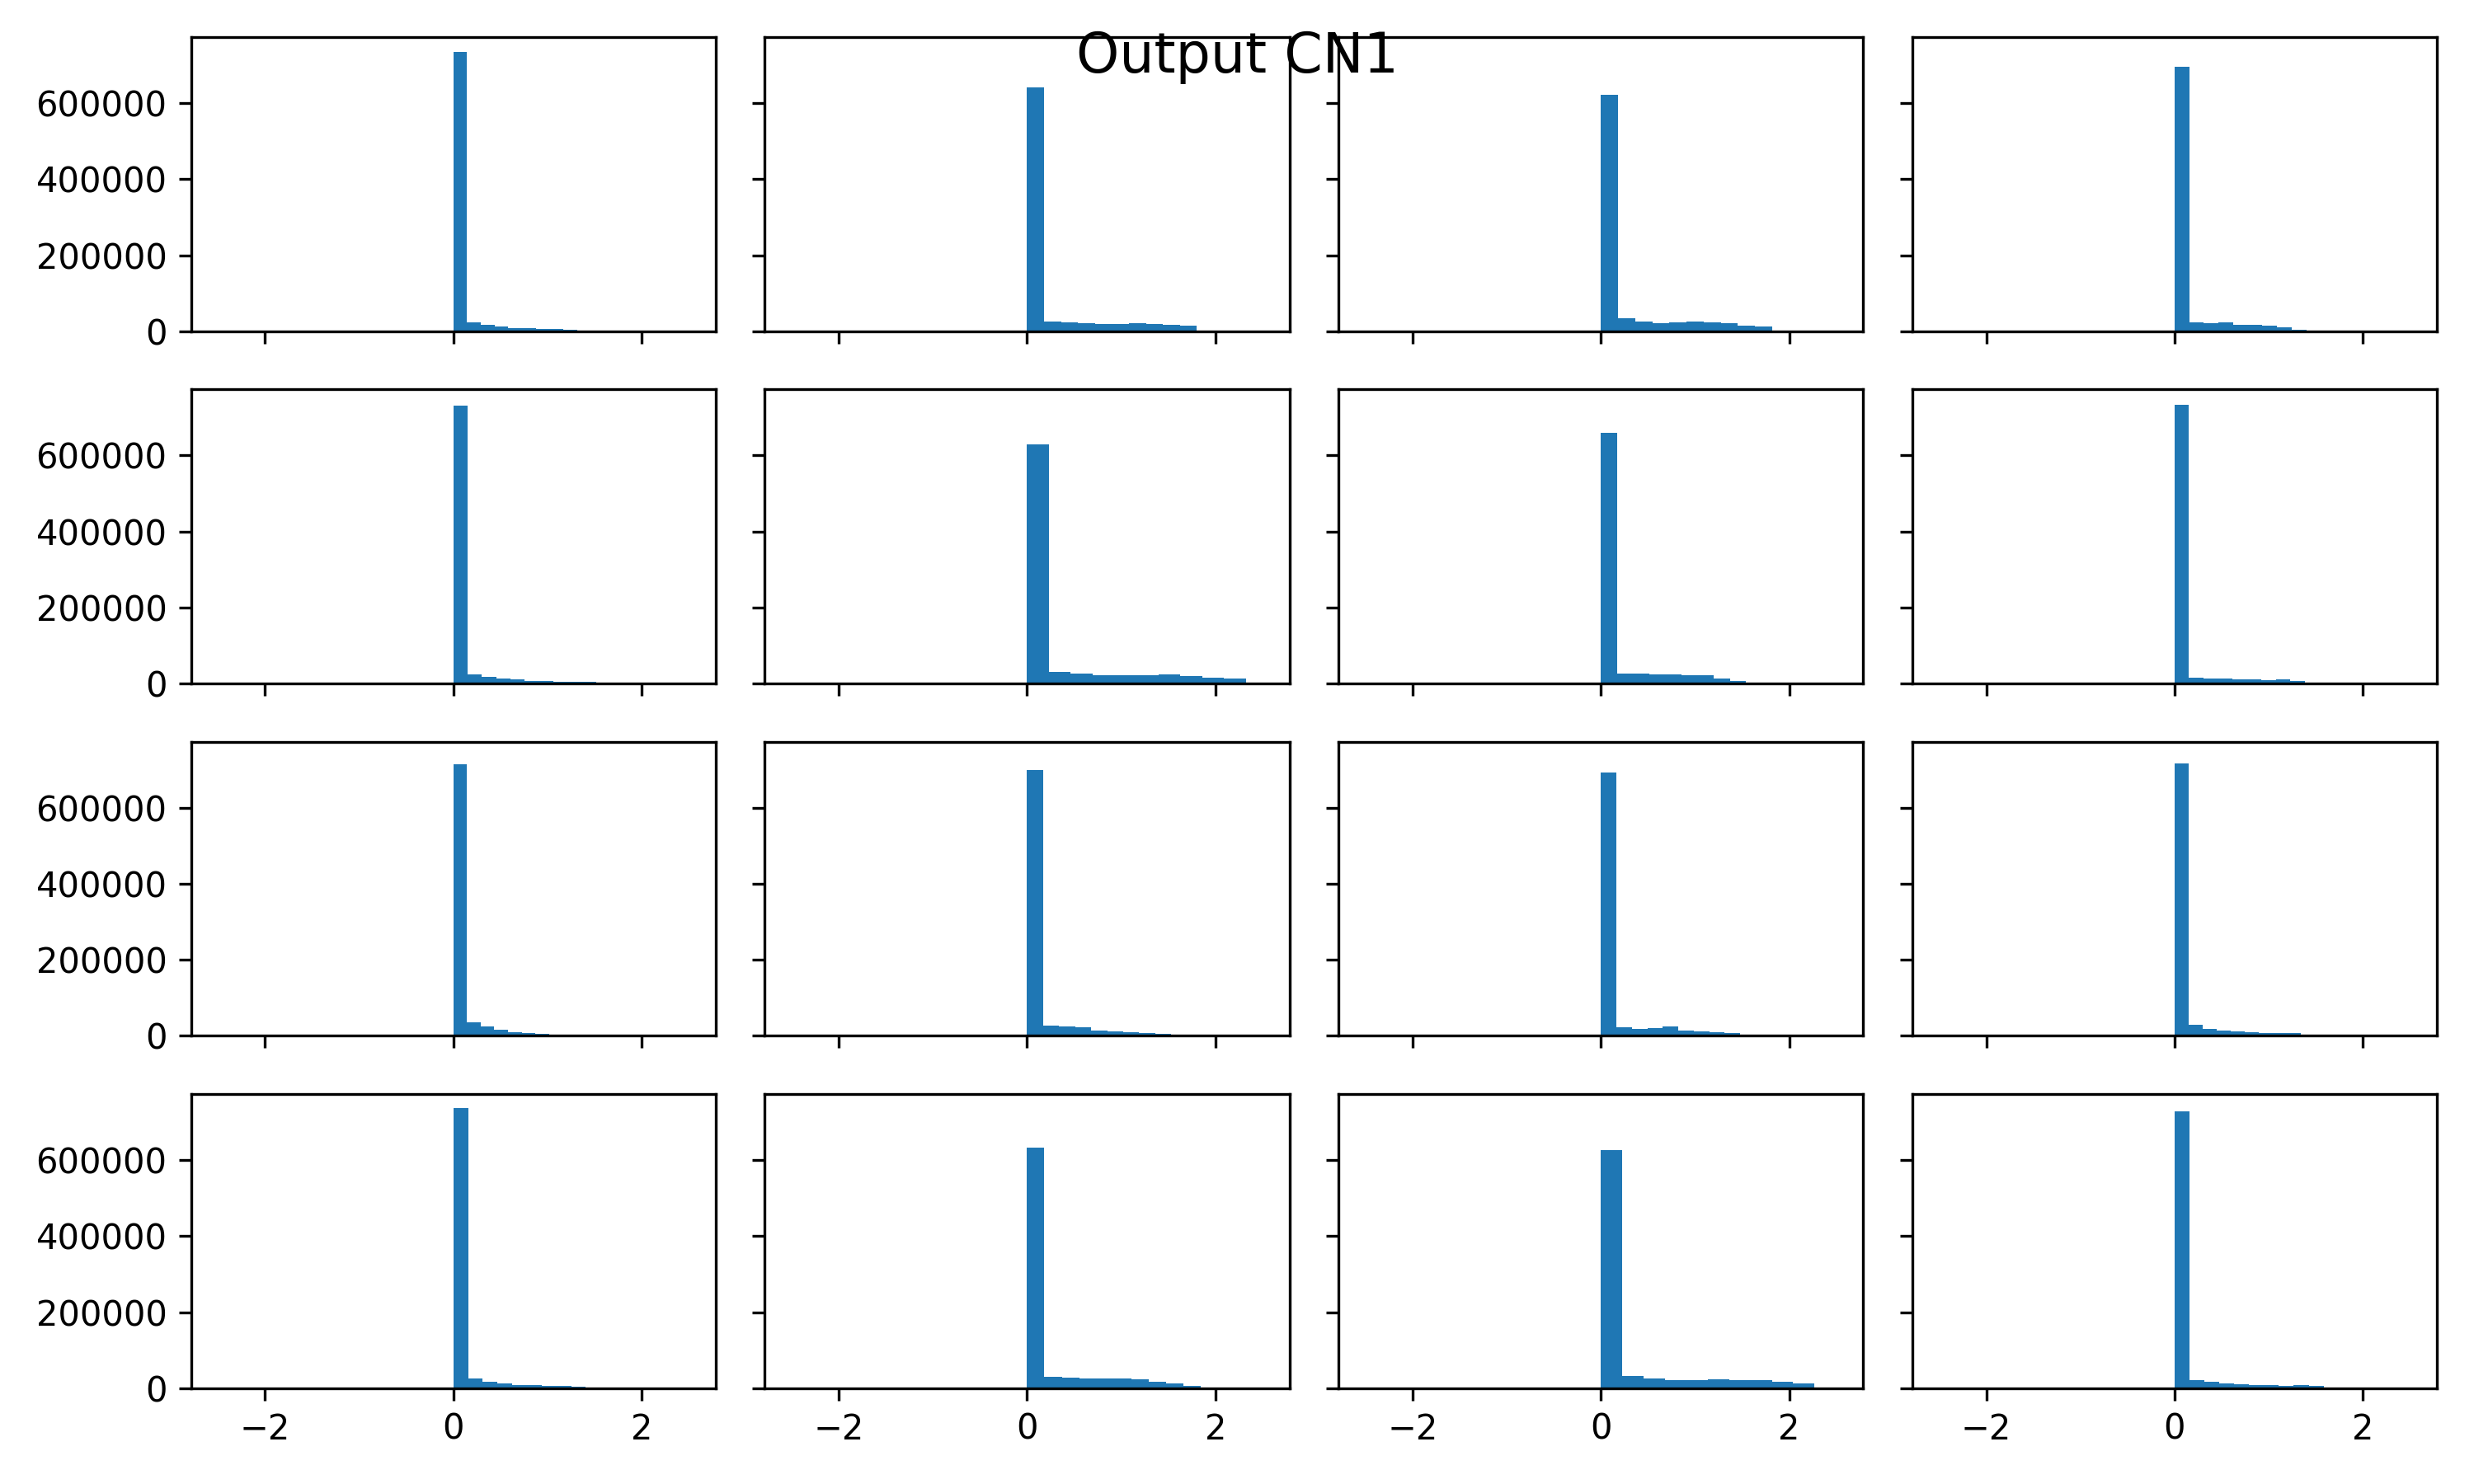
\includegraphics[height=1.6in]{../../net/images/hist_ao1}
        \caption{Convolutional Layer 1}
    \end{subfigure}%
    ~ 
    \begin{subfigure}[t]{0.5\textwidth}
        \centering
         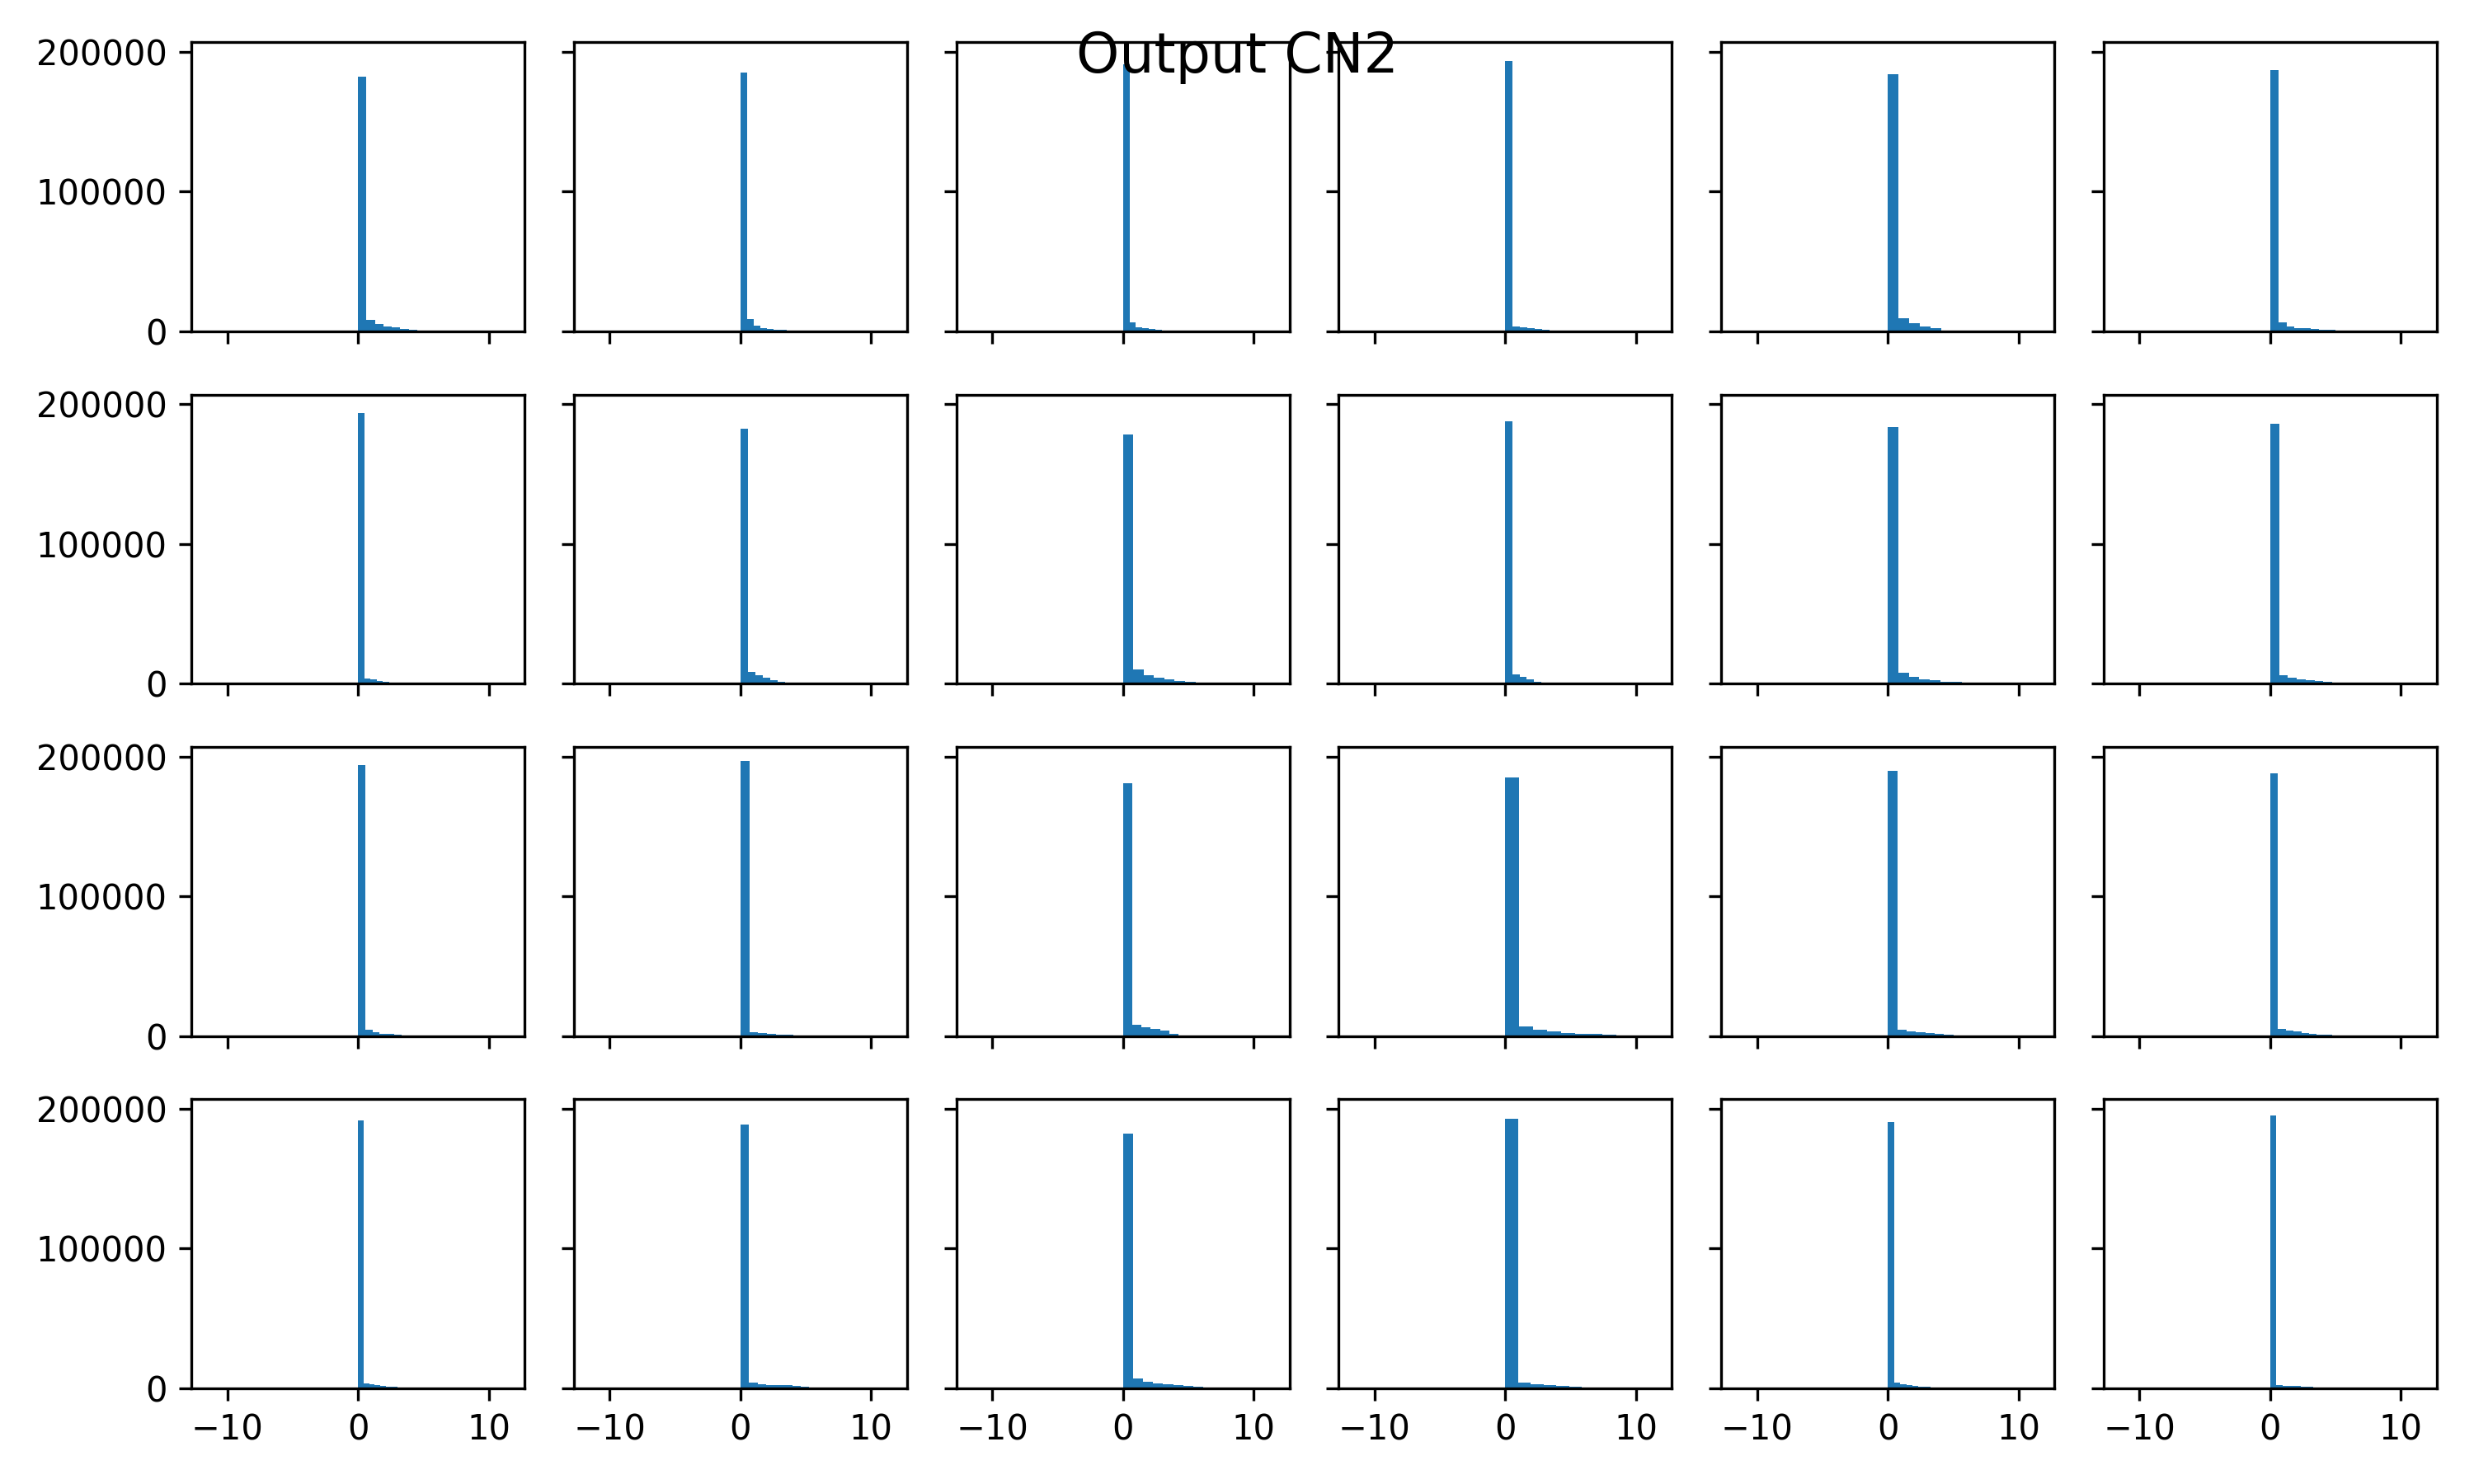
\includegraphics[height=1.6in]{../../net/images/hist_ao2}
        \caption{Convolutional Layer 2}
    \end{subfigure}%
    \\
    \begin{subfigure}[t]{0.5\textwidth}
        \centering
        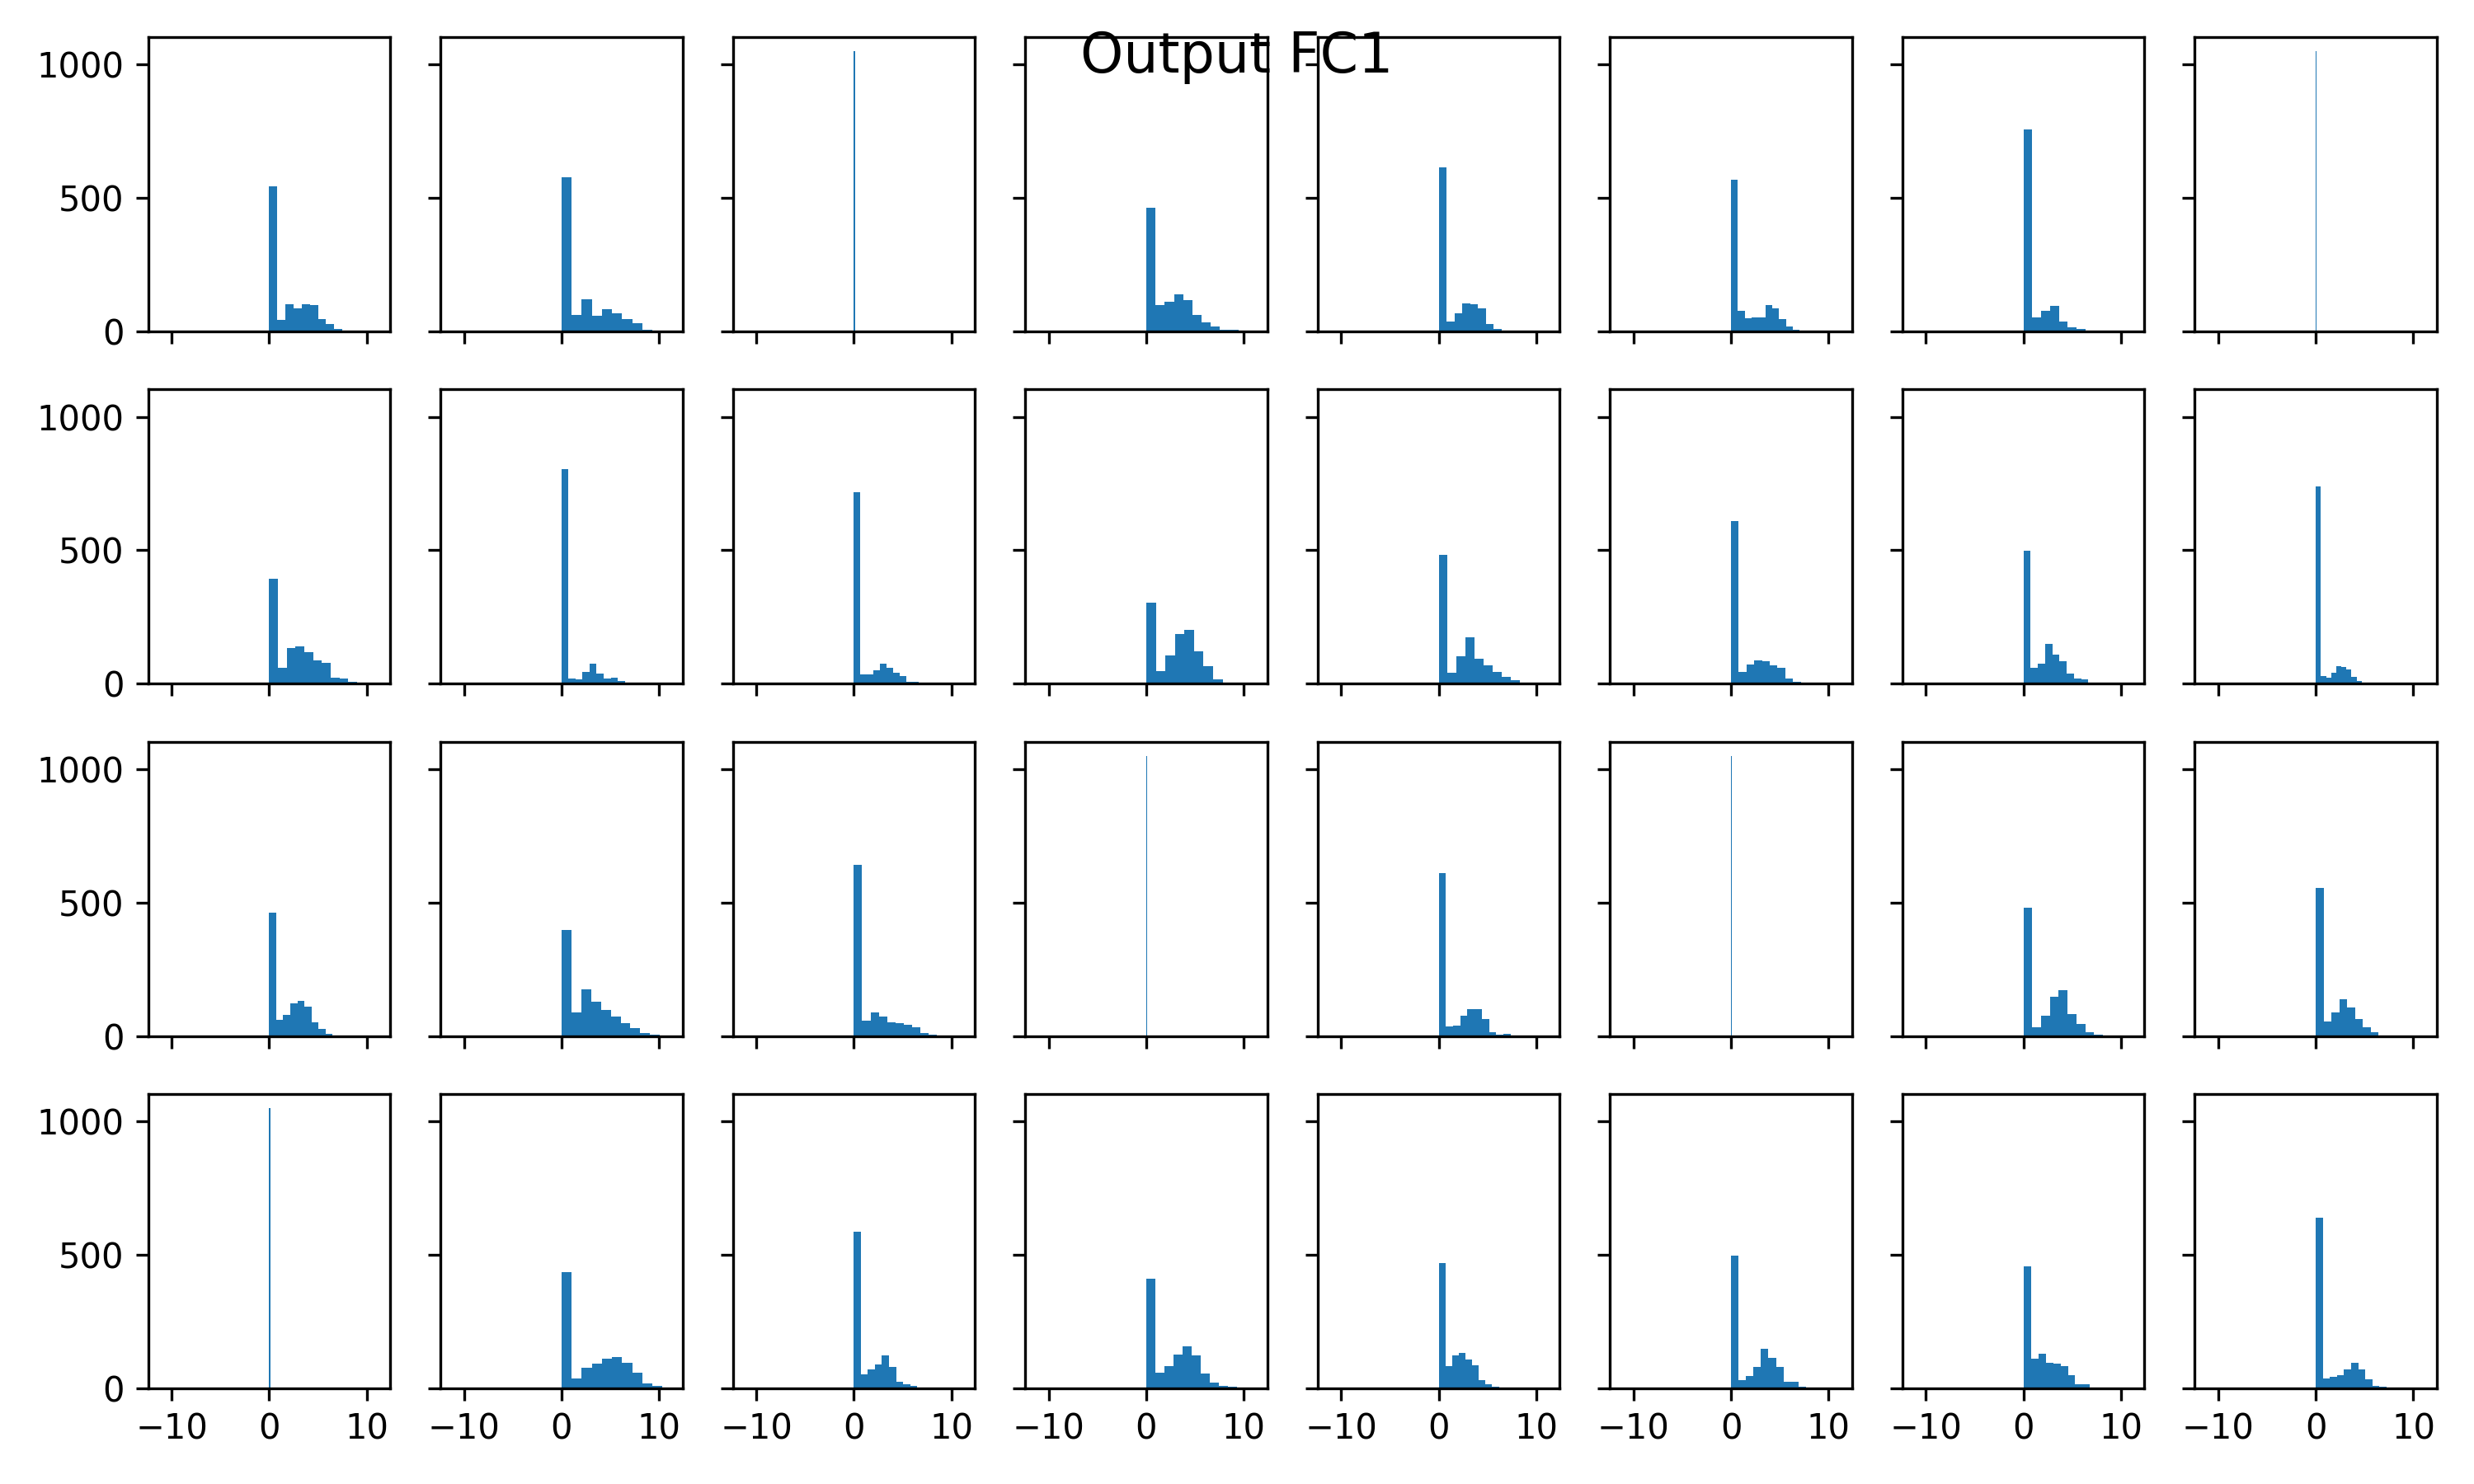
\includegraphics[height=1.6in]{../../net/images/hist_ao3}
        \caption{Fully Connected Layer 1}
    \end{subfigure}%
    ~ 
    \begin{subfigure}[t]{0.5\textwidth}
        \centering
         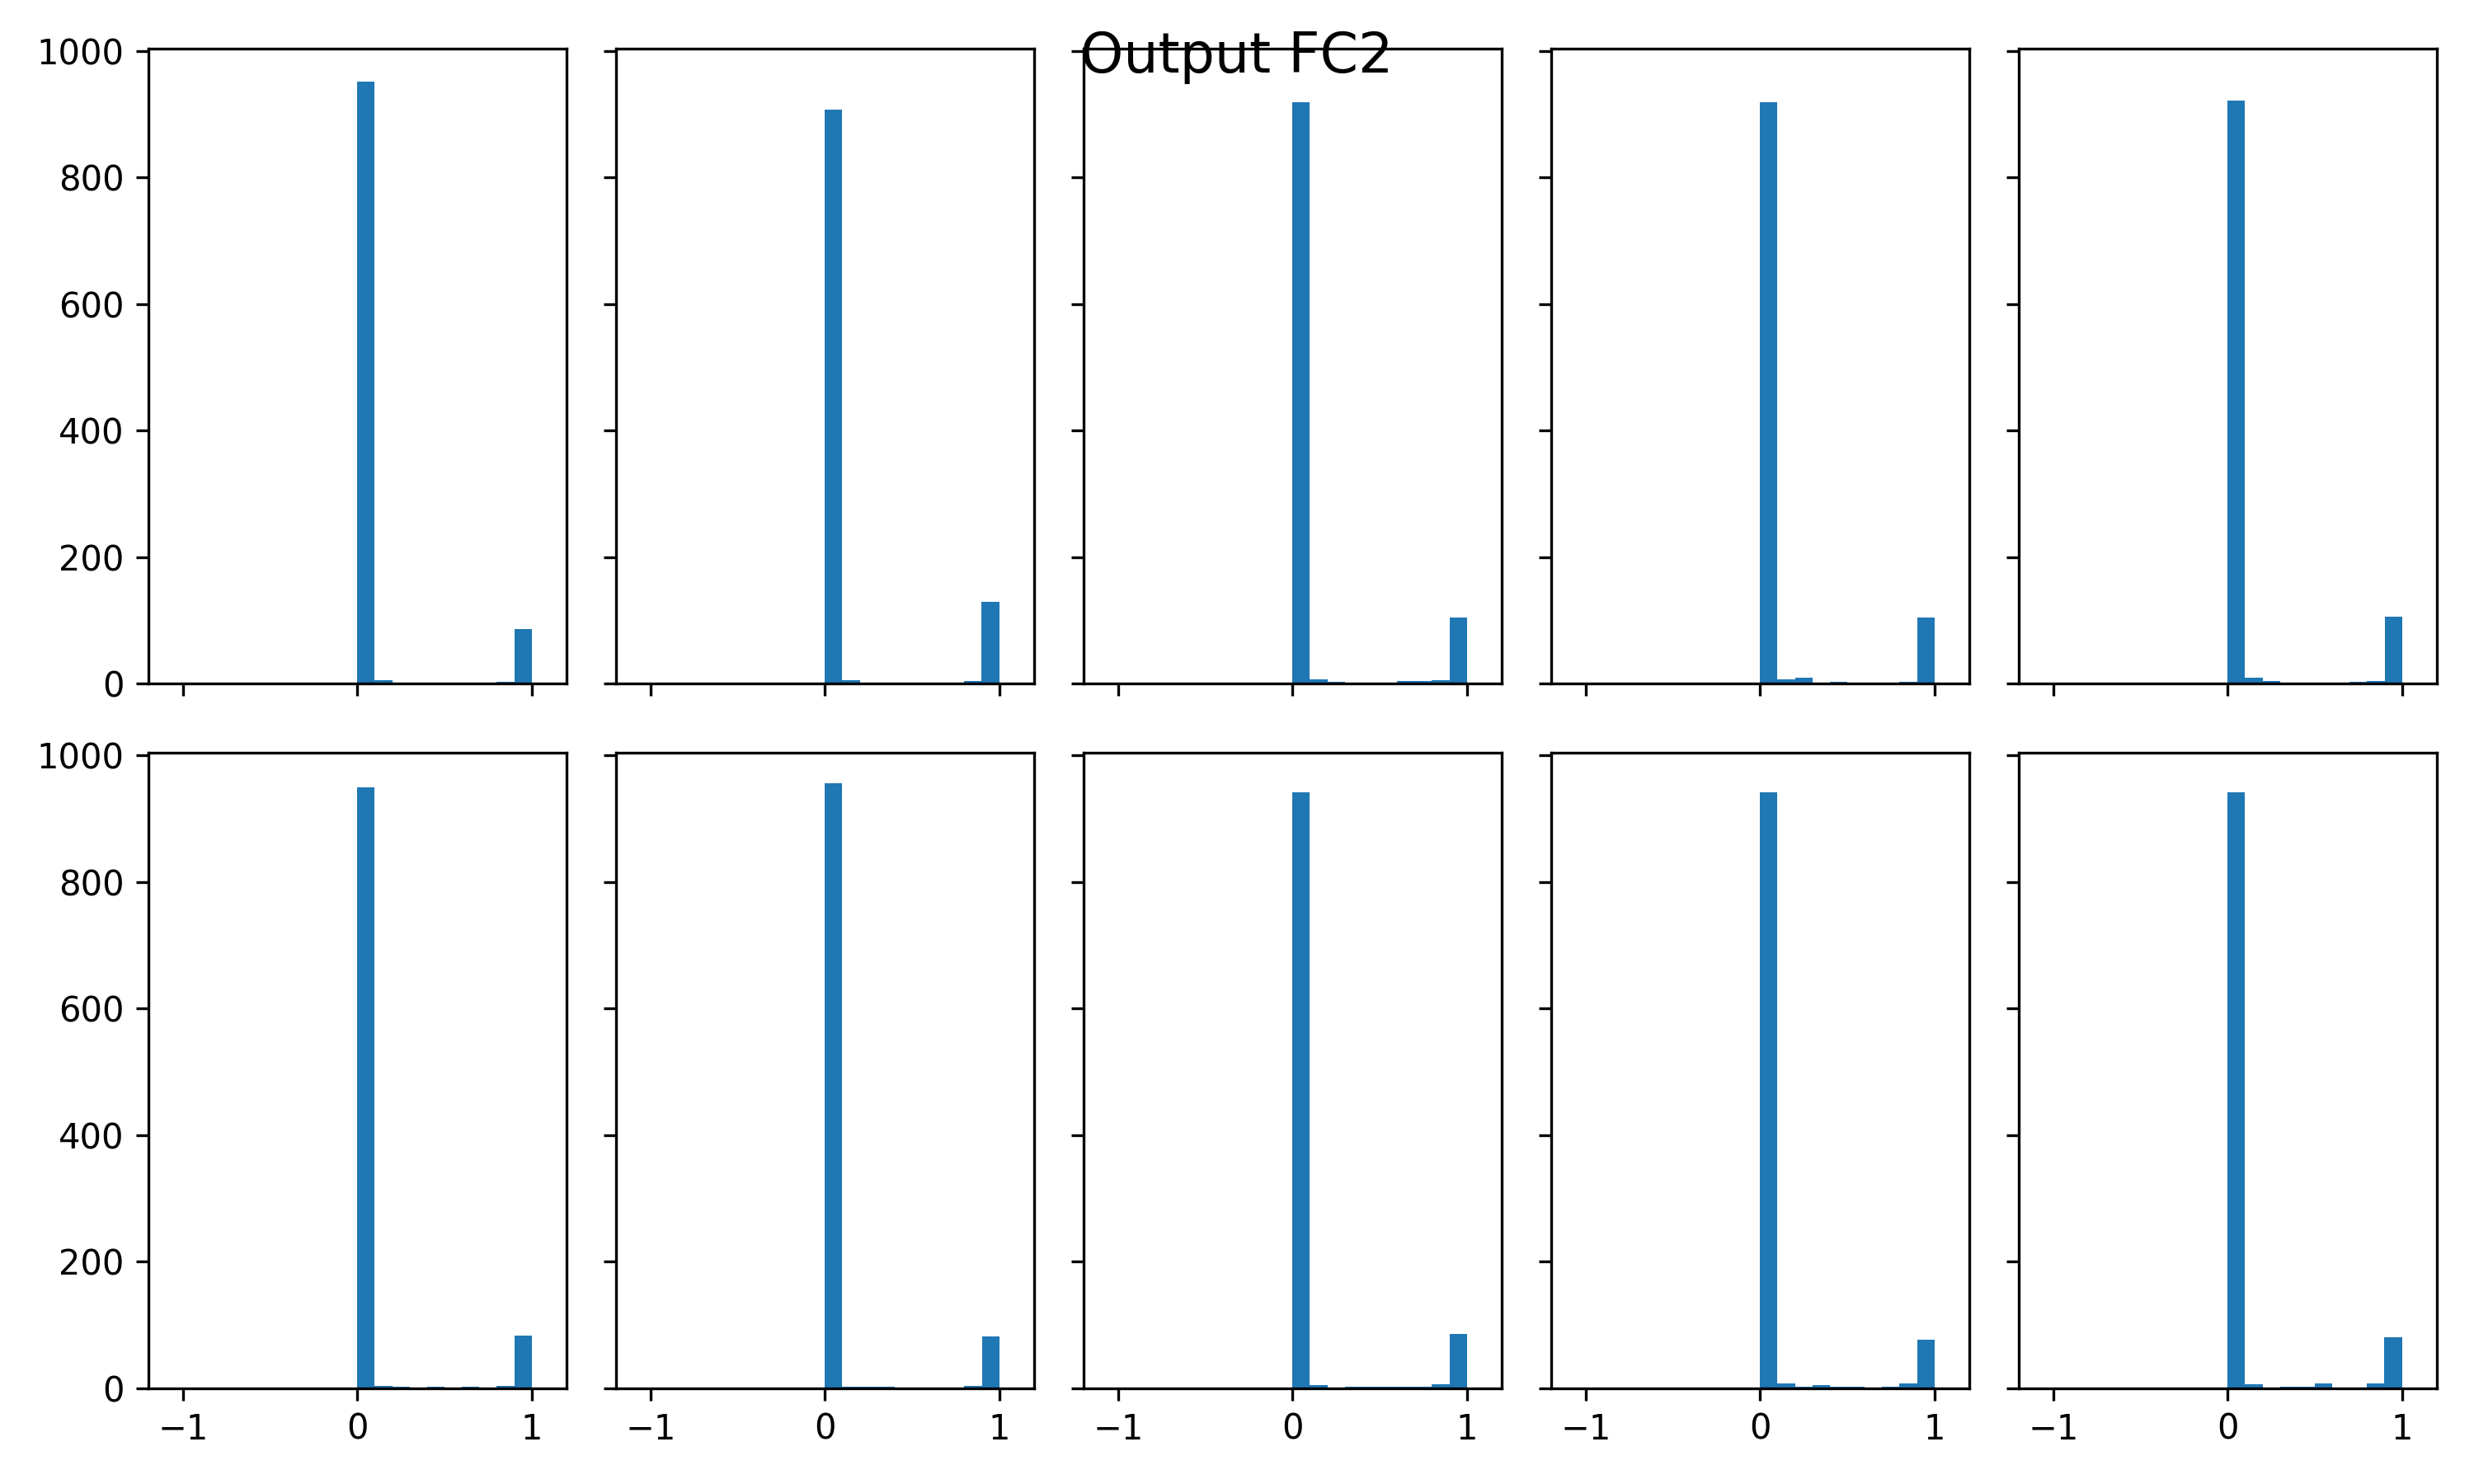
\includegraphics[height=1.6in]{../../net/images/hist_ao4}
        \caption{Fully Connected Layer 2}
    \end{subfigure}
    \caption{Distribution of the activations for a randomly selected batch of the input data}
    \label{fig:network-activations-distributions}
\end{figure}


\section{Software}

The remote software is either implemented on a PC or on a server. It is used for performing the training of the network and for generating a FPGA-bitstream based on the computed weights. Additionally the remote software is used to send the image data to the Zedboard and receive the results of the network for each image. 

Therefore the Host software can be separated in two parts:
\begin{itemize}
	\item Trainings software
	\item Communication software
\end{itemize} 

Requirements of the Trainings Software:
\begin{itemize} 
	\item Training of the network considering bit resolution of implemented hardware
	\item Create VHDL code based on the network hyper-parameter and on the computed weights
	\item Create a bitstream with the generated VHDL code
\end{itemize}

Requirements of the Trainings Software:
\begin{itemize}
	\item Sends image data to Zedboard
	\item Receives results from Zedboard
	\item Create a figure of accuracy and performance   
	\item Optional: Send bitstream to hardware which updates the bitstream 
\end{itemize}

\subsubsection{Interface to Zedboard} \label{subsec:InterfaceRemoteZed}
Ethernet is used for the communication of the remote host system and the embedded Linux which is running on the Zedboard. 
The embedded Linux distribution running on the board should automatically receive an IP address when connected to a network. When in doubt the address can be found out with the \texttt{ifconfig} command. 
The software has a client-server model with the embedded system acting as a server and the host as a client. Once running, the server software is listening for new outside connections. Different types of data need to be transmitted:

\begin{itemize}
	\item The 28x28 input images showing digits between 0 and 9 is transferred from host to Zedboard.
	\item The probability of resulting numbers between 0 and 9 is transmitted from Zedboard to host.
	\item control and status signals in both directions 
	\item Optional: Bitstream file for dynamically update the bitstream at the Zedboard
\end{itemize}

\subsubsection{Notes}
On Windows host systems, \emph{Network Discovery} needs to be enabled and in some cases a Firewall exception for the used ports needs to be set for a connection to be established. \\



\section{Hardware}
\subsection{Hardware Notation}


Generic Layer Interface

\begin{table}[h!]
\centering	
\begin{tabular}{l|cl}
	\toprule
	Parameter Name 		   	   & VHDL Type  & Description 								\\
	\midrule
	\texttt{s\_Clk\_i} 	       & \stdlogic  & Clock input								\\
	\texttt{s\_n\_Res\_i}.     & \stdlogic  & Reset input (active low)					\\
	\texttt{s\_Valid\_i} 	   & \stdlogic  & Flag, if the input is valid				\\
	\texttt{s\_Ready\_i} 	   & \stdlogic  & Flag, if the 								\\
	\texttt{s\_Last\_i} 	   & \stdlogic  & the parameter of the neural network		\\
	\bottomrule
\end{tabular}
\caption{Neural Network Layer Interface for VHDL Entities}
\label{tab:hw-layer-interface}
\end{table}


\subsection{Memory Controller}
The task of the memory controller is to provide valid data for the NN-layers in every cycle. It receives data from the previous layer of from the DMA and stores it in a Block-RAM. If a full image or feature map is received. The memory controller starts sending the data to the next layer. Receiving and sending data is performed in parallel, which therefore doesn't lead to additional delay time.  In order to read the $3\times3$ kernel in every clock cycle a linebuffer is used to store 2 lines. This enables the memory controller to provide a $3\times1$ vector in every cycle. To get a $3\times3$ kernel additionally a shiftregister is used.  

\subsubsection{Interfaces}
\begin{itemize}
	\item S\_LAYER: interface to previous layer
	\item M\_LAYER: interface to next layer 
	\item AXI\_lite: interface to AXI lite bus, is used to read BRAM data directly from processor (slow)
\end{itemize}

\subsubsection{Parameter}
\begin{itemize}
	\item BRAM\_ADDR\_WIDTH: integer: Address width of the connected Block-RAM
	\item DATA\_WIDTH: integer: Data width of activations
	\item IN\_CHANNEL\_NUMBER: integer: Number of input channels 
	\item LAYER\_HEIGTH: integer: Height of input matrix 
	\item LAYER\_WIDTH: integer: WIDTH of input matrix 
	\item AXI4\_STREAM\_INPUT: integer: 1 for input layer else 0 
	\item MEM\_CTRL\_ADDR: integer: Layer number of memory controller (used for AXI-lite interface)
	\item C\_S\_AXIS\_TDATA\_WIDTH: integer: AXI-stream data width (required for input layer)
	\item C\_S00\_AXI\_DATA\_WIDTH: integer: AXI-lite data width 
\end{itemize}

\subsection{AXI lite interface}
It is used to read the BRAM data directly from the processor which can be used for debug purposes. Each memory controller is assigned a unique address via generics in VHDL. One \SI{32}{\bit} register of the AXI lite bus is used for all memory controller. If the processor writes all 0 to the register, debugging mode is deactivated.  Therefore the memory controller address start with 1 and not with 0.
the \SI{32}{\bit} are separated as follows: \\
\begin{itemize}
	\item 23 downto 0: BRAM address
	\item 27 downto 24: \SI{32}{\bit} vector address 
	\item 31 downto 28 : Memory controller address 
\end{itemize}  

\begin{table}[hbt]
  \centering
  \begin{tabular}{l|lp{3in}}
    \toprule
    				              & Bit Address & Comment\\
    \midrule
    BRAM 				  & 23 downto 0  & Address of the block RAM \\
    \SI{32}{\bit} vector  & 27 downto 24 & If the width of one BRAM register is higher than \SI{32}{\bit}, the \SI{32}{\bit} vector address can be used to select the required part of the vector.\\
    Memory controller  	  & 31 downto 28 & Address of the memory controller used in the network starting with 1. If the address of the memory controller is selected debug mode is active. \\
    \bottomrule
  \end{tabular}
  \caption{AXI Lite component Address}
\end{table}




BRAM address: address of the block ram \\
\SI{32}{\bit} vector address: If the width of one BRAM register is higher than \SI{32}{\bit}, the \SI{32}{\bit} vector address can be used to select the required part of the vector. \\
Memory controller address: address of the memory controller used in the network starting with 1. If the address of the memory controller is selected debug mode is active. \\

 
\subsection{Convolutional Layer}

The convolutional layer - referred to as conv2d - receives an input data tensor $X_{ci} $ of size $[H, W, C_{in}]$ and outputs a data tensor of size $[H,W,C_{out}]$. Here $H$ and $W$ is the height and width of the convolutional kernel. So every input tensor is transferred to each single convolutional computation channel, which is responsible for computing a \emph{single} output channel. Each convolutional channel parameterized for with its own set of values. Those values are implemented as constants in VHDL, which has the advantages of greater optimization options by the compiler as well as reduced data movement. Therefore template entities are created where the weights are then populated via a Python script.

\begin{figure}[hb]
	\centering
	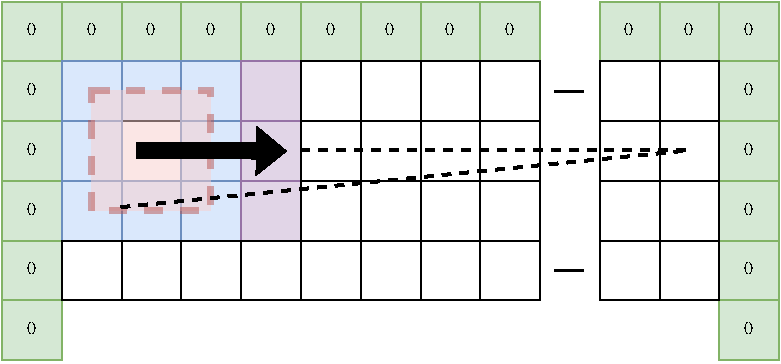
\includegraphics[width=0.6\textwidth]{img/convolution}
	\caption[Convolution Operation]{Convolution Operation. The convolutional kernel (red-dashed-square) is shifted over the input data. The currently processed data is shown in blue and the only three pixels (violett) need to be loaded for the next convolution because of data reuse. Note that for the convolution operation the image must be padded (in our case by zeros) to sustain image dimensions. Depth channels omitted for illustration purposes.}
	\label{fig:hw-conv-operation}
\end{figure}

The principal operation can be shown in Figure~\ref{fig:hw-conv-operation}. Here the convolutional kernel slides over the input data from left to right, top to bottom. It can be seen that most of the $6$ of $9$ input pixels (of each input channel) can be reused. This is done via shift registers and because all weights of the kernel remain unchanged for the operation this results in minimum data movement. Note that for the convolutional operations the input data must be padded in order to sustain the image dimensions.


\begin{figure}[h]
	\centering
	\begin{subfigure}[t]{0.5\textwidth}
		\centering
		% Constrain the height instead of the widht so the images are equally aligned at the top
		\includesvg[height=2.5in]{img/inkscape/conv2d.svg}
		\caption[Conv2d block diagram.]{Conv2d block diagram. For each output channel a conv\_channel module is used. $k$ indicates the number of output channels.}
		\label{fig:conv2d}
	\end{subfigure}%
	~
	\begin{subfigure}[t]{0.5\textwidth}
		\centering
		\includesvg[height=2.5in]{img/inkscape/conv-channel.svg}
		\caption[conv\_channel block diagram.]{conv\_channel block diagram. For each input channel a kernel\_3x3 module is used. $n$ indicates the number of input channels.}
		\label{fig:conv-channel}		
	\end{subfigure}
	\caption{Block diagram of the Convolutional Layer}
	\label{fig:hw-layer-conv}
\end{figure}


In Figure~\ref{fig:conv2d} the block diagram of the top-level conv2d module is shown. It consists of $k$ conv\_channel modules to realise $k$ output channels. All conv\_channel modules recieve the same input vector $X_{c_i}$. 
The internal structure of a conv\_channel module is shown in Figure \ref{fig:conv-channel}. It uses $n$ kernel\_3x3 modules to realise $n$ input channels. All kernel\_3x3 modules get a different input vector $X_{c_{i1}}$ to $X_{c_{in}}$ which are $3 \times 3$ input matrices. All kernel outputs are summed up to one final value of length BIT\_WIDTH\_OUT.

\subsubsection{Interface}

\begin{itemize}
	\item Input interface connected to shift register, which consists of a $n \cdot 3 \times 3$ vector of values of length BIT\_WIDTH\_IN, in which $n$ is the number of input channels.
	\item Output interface connected to the pooling layer, which is a vector of $m$ values of length BIT\_WIDTH\_OUT, in which $m$ is the number of output channels.
\end{itemize}
Both input and output interfaces have ready, last and valid signals to control the flow of data.

\subsubsection{Parameter}

\begin{table}[hb]
	\centering
	\begin{tabular}{lcc}
		\toprule
		Parameter & VHDL Datatype & Type \\
		\midrule
		 BIT\_WIDTH\_IN & integer & Generic\\
		 BIT\_WIDTH\_OUT & integer & Generic \\
		 INPUT\_CHANNELS & integer & Generic\\
 	 	 OUTPUT\_CHANNELS & integer & Generic \\
		\bottomrule
	\end{tabular}
\end{table}




\subsubsection*{conv\_channel}


\textbf{Interface}
\begin{itemize}
	\item Input interface, same as conv2d.
	\item Output interface connected to the pooling layer, which is a value of length BIT\_WIDTH\_OUT.
\end{itemize}

\textbf{Parameter}
\begin{itemize}
 	\item BIT\_WIDTH\_IN : integer
 	\item KERNEL\_WIDTH\_OUT : integer, output bit width of the kernel\_3x3 module
 	\item BIT\_WIDTH\_OUT: integer
 	\item N: integer, number of kernels
 	\item OUTPUT\_MSB: integer, defines which of the $n$=BIT\_WIDTH\_OUT bits is the most significant bit
 	\item BIAS: integer, currently unused as bias seems to not be very important in the convolutional layers
\end{itemize}

\subsection{Max Pooling Layer}

After the convolutional layer a pooling layer is placed. This reduces the dimensionality of the data and introduces local non-linearity to the network, enabling it to achieve better function approximation. In our case the layer performs a max operation among a $2 \times 2$ image patch. This means that a 2-by-2 image patch is mapped to 1 output pixel and it's value is equivalent to the maximum value of the input image patch.
Because of the processing of the convolutional layer (see Figure~\ref{fig:hw-conv-operation}) a whole input image input row must be buffered before any processing can happen. Because the pooling layer requires a $2$-by-$2$ input window it is limited by the output of the convolutional layer. To increase throughput the convolutional layer could be parallelized by doing two convolutions at once at the cost of increased area size. Alternatively the pooling operation can be serialized by only operating on half the output channels of the convolutional layer at a time.

\begin{figure}[h]
	\centering
	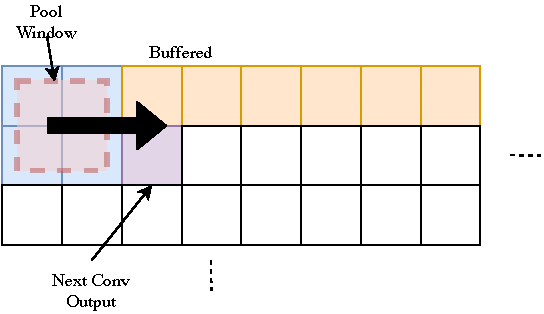
\includegraphics[width=0.6\textwidth]{img/pool.pdf}
	\caption[Pooling Operation]{Pooling Operation. The pool window (red-dashed-square) applied to current image patch (blue) and shifted over the input data. The first input row needs to be buffered (orange) before processing can happen. Depth channels omitted for illustration purposes.}
	\label{fig:hw-conv-operation}
\end{figure}

% TODO Finish table or dont use it at all
%\begin{table}[hb]
%	\centering
%	\begin{tabular}{lcc}
%		\toprule
%		Parameter & VHDL Datatype & Type \\
%		\midrule
%		 BIT\_WIDTH\_IN & integer & Generic	 	\\
%		 BIT\_WIDTH\_OUT & integer & Generic 	\\
%		 INPUT\_CHANNELS & integer & Generic 	\\
% 	 	 OUTPUT\_CHANNELS & integer & Generic 	\\
% 	 	 \midrule
% 	 	 valid\_i & \stdlogic & input \\
% 	 	 data\_i & \stdlogic[INPUT\_CHANNELS][DATA\_WIDTH] & input \\
% 	 	 \midrule
% 	 	 valid\_o & \stdlogic & output \\
% 	 	 data\_o & \stdlogic[INPUT\_CHANNELS][DATA\_WIDTH] & output \\
%   		\bottomrule
%	\end{tabular}
%	\caption{}
%	\label{tab:hw-pool-layer-parameter}
%\end{table}

\subsection{NN}

\subsubsection{Operation}
\begin{figure}[h]
	\centering
	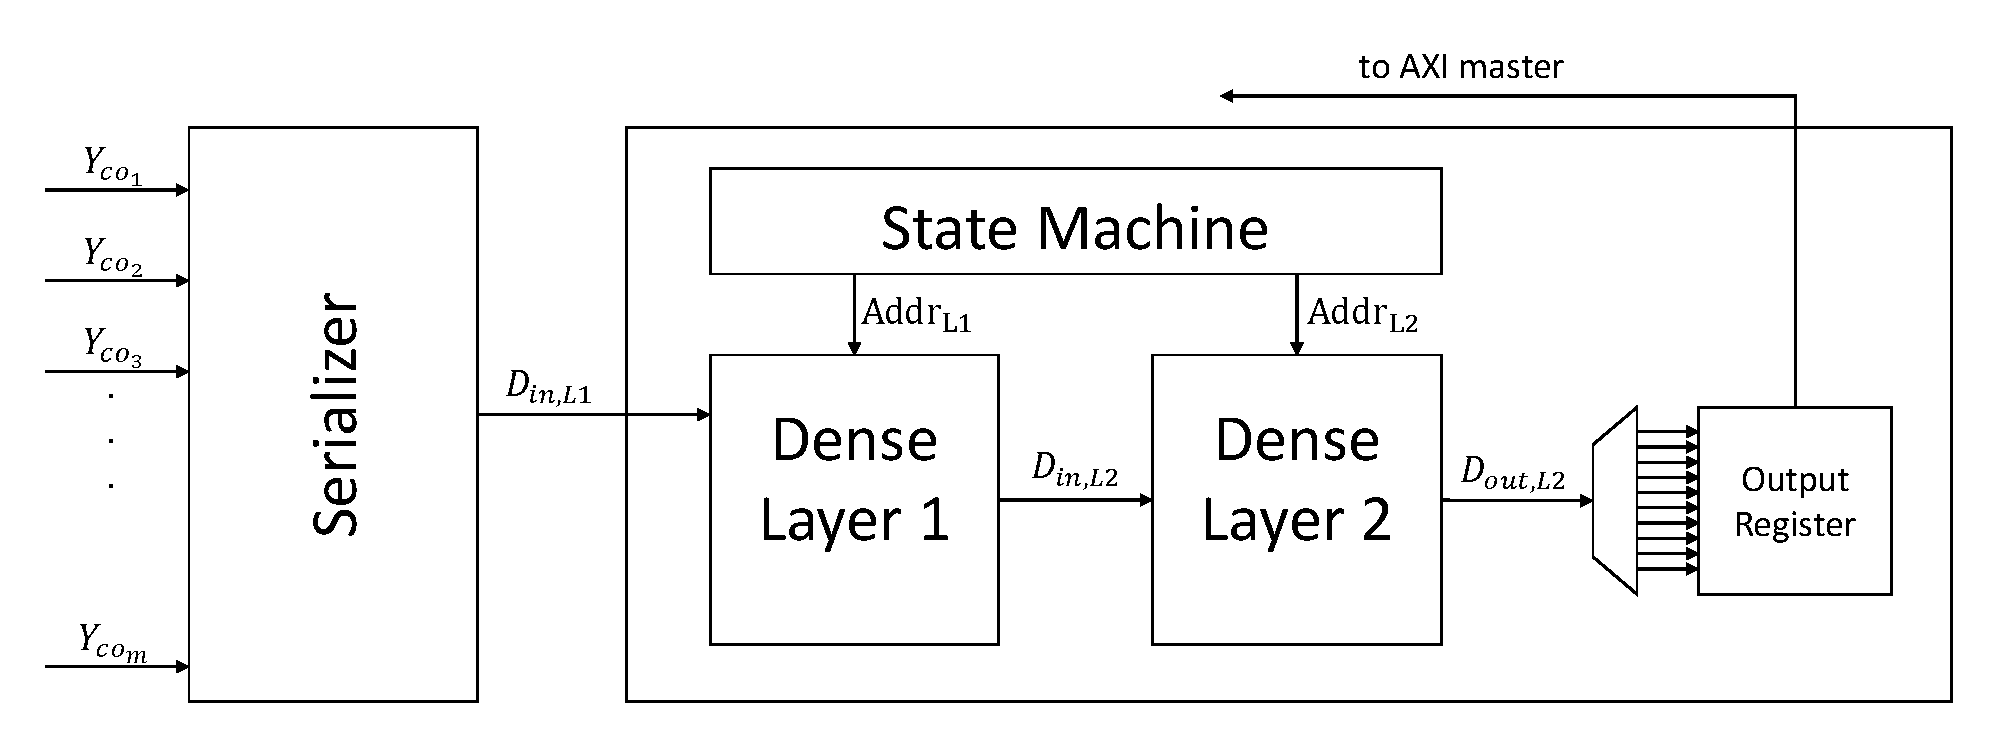
\includegraphics[width=0.8\textwidth]{img/dense.pdf}
	\caption{Diagram of the combined, fully connected NN.}
	\label{FIG:nn}
\end{figure}

The fully-connected neural network is shown in figure \ref{FIG:nn}. It consists of two dense layer instances controlled by a state machine. The output of layer 1 is fed directly into the layer 2. The output of layer 2 are 10 values which represent the confidence that the input image showed a specific number. 

The Serializer module is connected to the previous pooling layer. The $m=32$ output channels need to be converted into a stream of single values of length VECTOR\_WIDTH. For this, the previous pooling layer is stalled by keeping the ready signal low while a vector of $m$ values is serialized.

\subsubsection{Interface}
\begin{itemize}
	\item Input interface, a stream of values of length VECTOR\_WIDTH
	\item Output interface, a vector of 10 values of length VECTOR\_WIDTH
\end{itemize}
\subsubsection{Parameter}
\begin{itemize}
	\item VECTOR\_WIDTH: integer
	\item INPUT\_COUNT: integer
	\item OUTPUT\_COUNT: integer
\end{itemize}
\subsection{Dense Layer}
\label{sec:hw-fully-connected}

\subsubsection{Operation}
\begin{figure}[h]
	\centering
	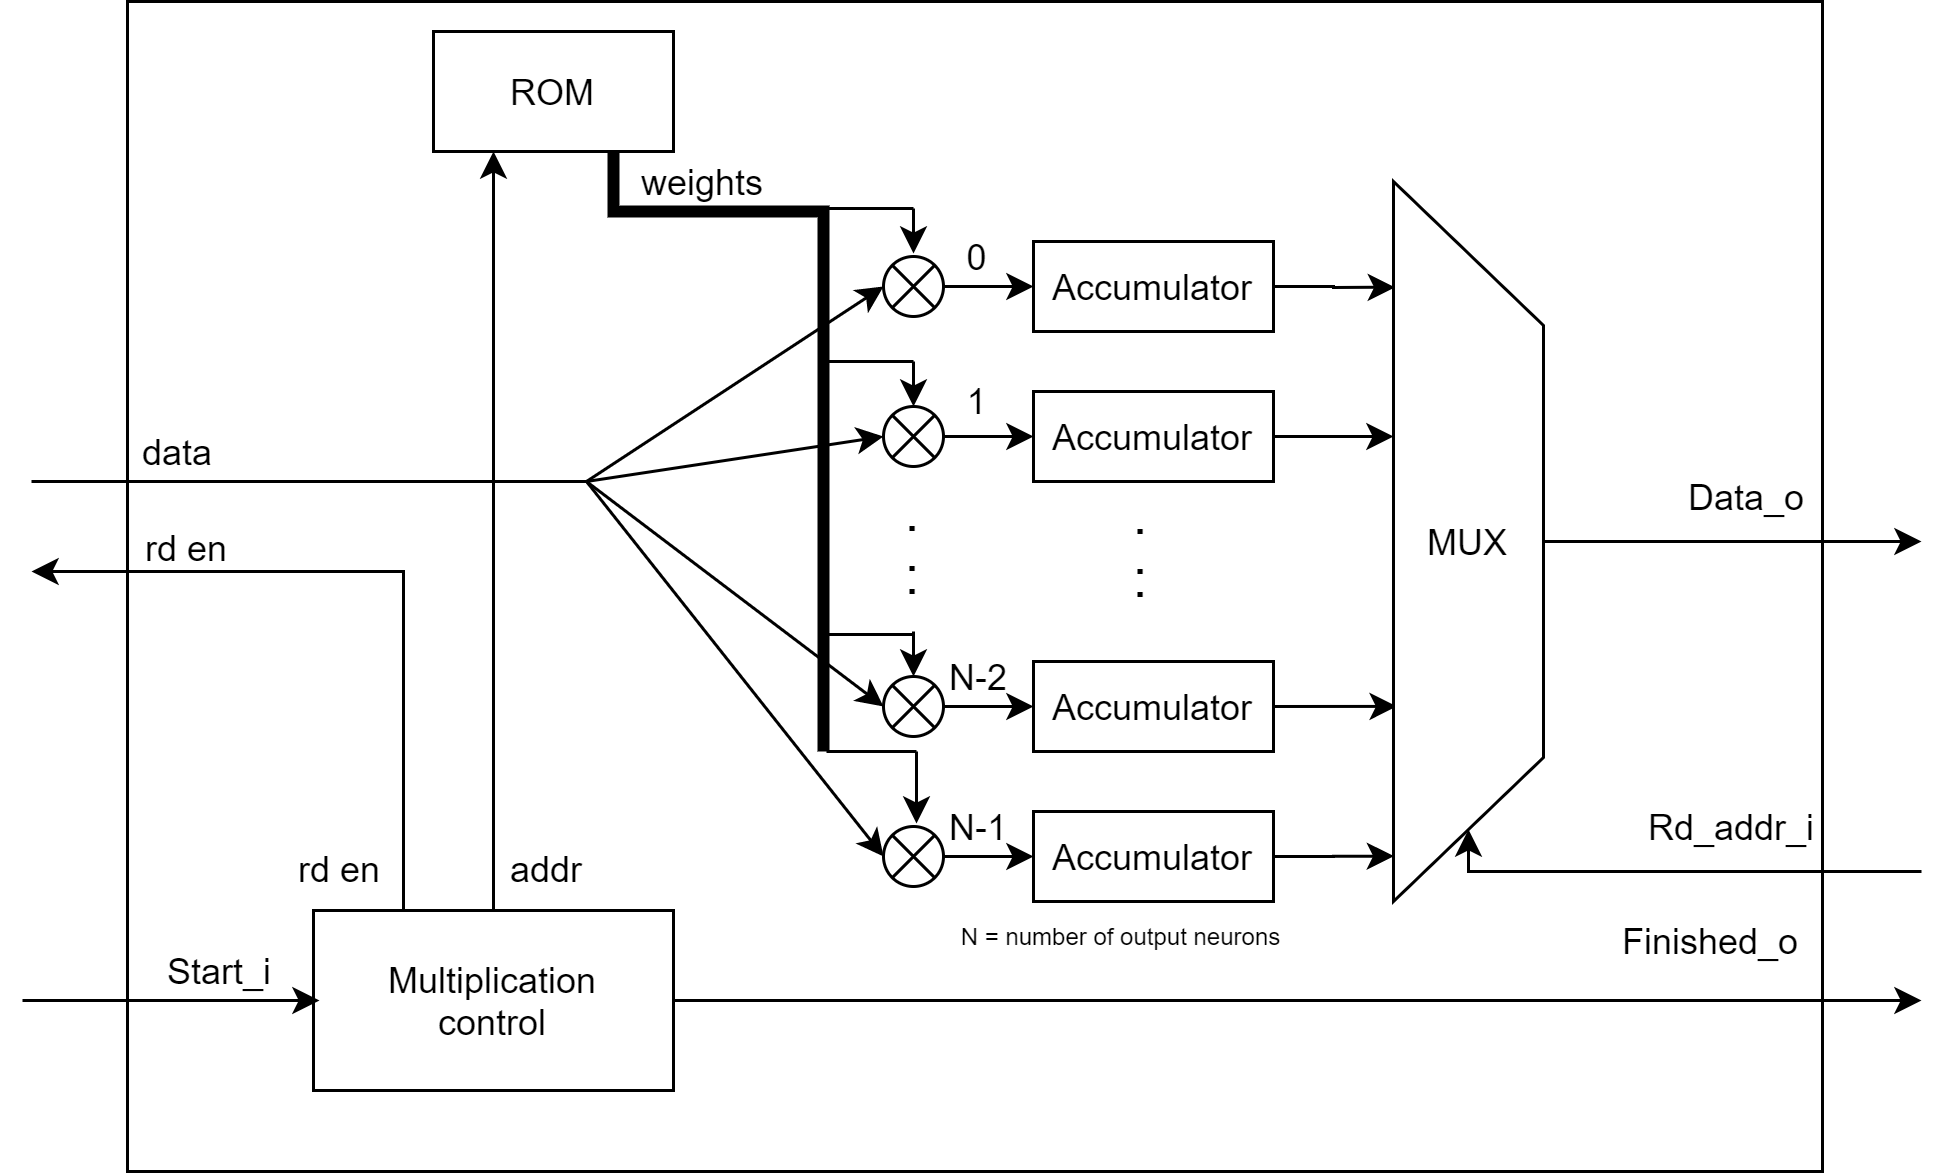
\includegraphics[width=0.8\textwidth]{img/blockDiagramDense.png}
	\caption[Dense layer diagram]{Dense layer diagram.}
	\label{fig:denseLayerBlockDiagram}
\end{figure}

Figure~\ref{fig:denseLayerBlockDiagram} depicts the dense or fully connected layer of the network. This block contains a finite state machine. When the Start\_i input port goes high, input neurons are read from an external ROM one by one. Each of the input neurons is multiplied by appropriate weight for each of the output neurons. The products are then fed into accumulators, which calculate a sum of all products of all neurons with the inputs. When all of the incoming neurons are processed, the calculation is finished and a Finished\_o signal is raised high to signal that data is available. Result data can be addressed by Rd\_addr\_i port and read out at the Data\_o port.

Number of input neurons, output neurons and data width are generic.

\subsubsection{Weights}

Weights are stored in a ROM memory. The values are hardcoded at synthesis. The VHDL code reads the weights from a file. File contains the weight values in binary. Each line represents all of the weights for one input neuron. There are as many lines as there are input neurons.

\subsubsection{Bias terms}

Bias terms are also loaded from a file. Each output neuron has its own bias term. Each line contains one bias term. Bias term bit width is generic. Bias terms are treated as a signed value.
	

\subsubsection{Parameters}
\begin{description}
	\item [VECTOR\_WIDTH   : integer] Bit width of input data.
	\item [INPUT\_COUNT    : integer] Number of input neurons
	\item [OUTPUT\_COUNT   : intege] Number of output neurons.
	\item [ROM\_FILE       : string] File, that holds the weight values.
	\item [BIAS\_WIDTH     : integer] Bit width of the bias terms.
	\item [BIAS\_FILE      : string] File, that holds the bias term values.
\end{description}




%\section{Conclusion}



\section{Appendix}
\input{09_build}
\subsection{Network Operations}
\subsubsection*{Convolutional Operations}

The output of an convolutional layer is defined by
\begin{equation}
   z(i,j) = (f*g)(i,j) = \sum_{m=-\infty}^{\infty} \sum_{n=-\infty}^{\infty} f(m,n) g(m-i,n-j)
\end{equation}

It is explained in more detail here: \cite{dumoulin2016guide}

\subsubsection*{Fully Connected Layer}

The output of an fully connected layer is defined by
\begin{equation}
	z = xW + b
\end{equation}
where $x \in \mathbb{R}^{b,m}$,  $W \in \mathbb{R}^{m,n}$ and $b \in \mathbb{R}^{n}$. 

\subsubsection*{Rectified Linear Unit (ReLU)}

\begin{equation}
	f(x) = \begin{cases}
		x \quad \text{if} \quad x > 0 \\
		0 \quad \text{else}
	\end{cases}
\end{equation}


\subsubsection*{Softmax}

\subsection{Matrix Calculus}

The chain rule for a vectors is similar to the chain rule for scalars. Except the order is important. For $\mathbf{z} = f(\mathbf{y})$ and $\mathbf{y} = g(\mathbf{x}) $ the chain rule is:
\begin{equation}
    \frac{\partial \mathbf{z}}{\partial \mathbf{x}} = \frac{\partial \mathbf{y}}{\partial \mathbf{x}}     \frac{\partial \mathbf{z}}{\partial \mathbf{y}}
\end{equation}




\begin{table}[h]
    \centering
    \begin{tabular}{cc}
        \toprule
            $y$ & $\frac{\partial}{\partial x} y$ \\
        \midrule
            $Ax$     & $A^T$ \\
            $x^T A$  & $A$   \\
            $x^T x$  & $2x$  \\  
            $x^T Ax$ & $Ax + A^Tx$  \\          
        \bottomrule
    \end{tabular}
    \caption{Useful derivatives equations}
\end{table}


\subsection{Fix-Point Arithmetic}

Multiplication of two fix point values yields 
\begin{equation}
	v_1 v_2 = \text{right-shift}\left( Q_1 Q_2 \cdot 2^{-(m+m)} ; m\right)
\end{equation}
Note that for multiplication the exponent $m$ for the values can be different.

Addition of two fix point values
\begin{equation}
	v_1 + v_2 = \left( Q_1 + Q_2 \right) \cdot 2^{-m}
\end{equation}
\subsection{Source Code}

All the source code is licensed under the \emph{MIT} Licence and can be found on Github.
\url{https://github.com/marbleton/FPGA\_MNIST}

There are also the most up to date build instructions how to compile the project. Those are in short:

Dependencies
\begin{itemize}
	\item Vivado 2017.4
	\item Python 3.6 including Numpy \cite{Walt:2011aa}, SWIG \cite{Beazley:2003aa}, Keras \cite{Gulli:2017aa} and Torch \cite{Paszke:2019aa}
\end{itemize}

\begin{enumerate}
	\item Train the network using the \texttt{net/train\_keras.py} script
	\item Use the network \texttt{net/quant.py} script to quantize the trained network layers
	\item Generate the VHDL files
\end{enumerate}


\subsection{Other}

Other resources which are useful:

How Tensorflow is implementation \url{https://github.com/dmlc/nnvm-fusion} and \url{https://github.com/tqchen/tinyflow}

Deep Learning Course from University of Washington \url{http://dlsys.cs.washington.edu}


\listoffigures
\listoftables
%\listoftodos
\bibliographystyle{apalike}
\bibliography{bibhelper,references}


\end{document}
